\chapter{Quantization for Network State Modeling}
	\label{cha:quantization}
	
	When communicating with others, we often use the description of a single entity to describe the characteristics of a whole group.
	Using examples in this form is a very effective way of conveying information; the listener intuitively understands that the highlighted aspects are what distinguish the given group from the rest, while also keeping in mind that there are likely entities in the group with slightly differing attributes compared to the example given.
	Using examples are most important when describing a large amount of entities, in which case multiple examples are usually given to cover the whole range of attributes.
	However, selecting which examples to use in order to maximize their descriptiveness can be quite a challenge.
	
	\emphix{Quantization}{quantization} realizes this task as a \ac{ML} algorithm, in which a large number of observations with a continuous distribution (the dataset) are mapped to a small set of discrete observations (the examples/prototypes/centroids).
	Quantization algorithms split the input space into a finite number of partitions, and use a single observation from within each partition as an exemplary representation of all the observations in that partition.
	Just as in human communication, exemplification through quantization also serves the purpose of effective communication for machines, by maximizing the amount of useful information communicated with a minimum amount of data.
	Quantization algorithms are primarily used in signal processing, where their task is to remove minute variance from the data, and compress the information into the smallest possible encoding, which can then, e.g., be transmitted over radio, or effectively stored on a hard drive.
	
	Quantization is not to be confused with clustering; while in clustering, the goal is to find originally present groups in the data, quantization only aims to partition the data into possibly arbitrary parts, in order to effectively compress information.
	Quanta do not necessarily adhere/align to clusters in the data, because in most use cases, the quantization will use far more quanta than the number of groups present.
	However, as we will see later, good quantization algorithms do have to take into consideration clusters in the data, thus blurring the division between clustering and quantization algorithms.
	
	Communication through examples is also useful in network automation, where the quanta can be seen as \emphix{network states}{network state}, which describe the settings, current performance, and/or context of single or multiple entities in the network, such as base-stations, gateways, cells, or even users.
	Network states are meant to form the basis of communication -- a vocabulary -- between cognitive functions in the mobile network, upon which control decisions or reconfiguration requests can be based.
	Because the mobile network is understood to be a dynamically changing context, it is important to have the network states automatically defined, so that in case of a context change, they can be quickly redefined without human supervision, making the management system adaptive to change.
	
	Sec.~\ref{cha:quantization:sec:knowledge_sharing} introduces the concept of knowledge sharing for self-healing -- which uses quantization and some form of network states -- through the following patent application:
	
	\begin{patent}
		Diagnosis Knowledge Sharing for Self-healing \\
		\textit{Benedek Schultz, Janne Ali-Tolppa, Márton Kajó} \\
		WO, PCT application no.: PCT/EP2018/079735, filed Oktober 2018
	\end{patent}

	Sec.~\ref{cha:quantization:sec:bvq} of this chapter is based on the work published in the following paper:
	
	\begin{publication}
		Equal-volume Quantization of Mobile Network Data using Bounding Spheres and Boxes \\
		\textit{Márton Kajó, Benedek Schultz, Janne Ali-Tolppa, Georg Carle} \\
		NOMS 2018-2018 IEEE/IFIP Network Operations and Management Symposium, pp. 1-9. IEEE, 2018.
	\end{publication}
	
	My contributions to the above paper was the design, implementation and evaluation of the algorithm, as well as the co-authoring of the paper.
	The discussion in this thesis expands on the paper, by placing it into the larger concept of knowledge sharing in self-healing, as well as the proposal of an alternative, neural-net-based implementation, published in the following report (Sec.~\ref{cha:quantization:sec:nn_quant}):
	
	\begin{publication}
		Neural Network-based Quantization for Network Automation \\
		\textit{Márton Kajó, Stephen S. Mwanje, Benedek Schultz, Georg Carle} \\
		arXiv preprint arXiv:2103.04764 (2021).
	\end{publication}

	My contribution to this technical report was the design, implementation and evaluation of the algorithm, as well as the authoring of the document itself.
	While containing important details for our future work, we deemed the content of this report to be too technical for a mobile-networks-oriented audience (please see Sec.~\ref{cha:conclusion:sec:dl_research} for further notes on this), thus, instead of publishing it as a scientific paper, the report was made freely available on arXiv.
	
	The overall discussion is concluded with some remarks on the complexities of implementing algorithms for massive parallelization, and integrating them into \ac{DL} frameworks or algorithmic pipelines, a topic which came up often in our research.

	Some of the findings from this work as are also echoed in the following publications (both of which I also co-authored, but no additional text is used from them in this dissertation):
	
	\begin{publication}
		Self-healing and Resilience in Future 5G Cognitive Autonomous Networks \\
		\textit{Janne Ali-Tolppa, Szilárd Kocsis, Benedek Schultz, Levente Bodrog, Márton Kajó} \\
		2018 ITU Kaleidoscope: Machine Learning for a 5G Future (ITU K), pp. 1-8. IEEE, 2018.
	\end{publication}

	\begin{publication}
		Cognitive Autonomy for Network Self‐Healing \\
		\textit{Janne Ali-Tolppa, Márton Kajó Georg, Borislava Gajic, Ilaria Malanchini, Benedek Schultz, Qi Liao} \\
		Towards Cognitive Autonomous Networks: Network Management Automation for 5G and Beyond (2020): 345-384.
	\end{publication}

	\section{Concept: Diagnosis Knowledge Sharing for Self-Healing}
		\label{cha:quantization:sec:knowledge_sharing}
		
		\subsection{Automating Diagnosis in Self-Healing}
			
			Network assurance relies largely on monitoring the alarms generated by network elements, or by monitoring their performance directly.
			Alarms are triggered through the process of \ac{FM}, where individual network elements monitor preset thresholds, and generate alarm messages if a threshold is overstepped.
			The diagnosis of discovered anomalies often relies solely on human inference.
			Given the complexity and growth of mobile networks, such processes do not scale, and will become infeasible in the near future.
			Consequently, there is a need for augmented processes in relation to networks for diagnosing network anomalies.
			In this context, augmented refers to processes where human inference is supplemented by \ac{ML}, in order to reduce labor and speed up processing, hopefully ultimately leading to full automation.
			At the time of this work, we had solutions for automated anomaly detection, but not for augmented or automated diagnosis.
			
			One of the main focuses of \ac{SON} is self-healing, where the goal is to automatically detect and correct faults in the network.
			The self-healing process can be split up into $3$ steps: the detection, diagnosis, and correction of faults.
			The deployment of corrective actions is a quite complicated topic, and has been researched extensively \cite{tsvetko_verif_1, tsvetko_verif_2}, thus it will not be discussed here, instead, this work focuses on the preceding step, the diagnosis of anomalies, for which the detection process has to be introduced.
			
			The detection of anomalies can be automated in a conceptually straightforward way \cite{anonamly_det}, by comparing the current performance to an established profile that describes the normal behavior of the network.
			These profiles are likely formed by \ac{ML} algorithms, such as neural nets.
			The profiles are created from \ac{PM} measurements of a set period, and can be updated either periodically or continuously to combat profile aging, thus creating resilience against false detections stemming from slow, trend-like changes in network behavior.
			The profiling and detection are done based on a set of selected features, e.g. \ac{PM} \acp{KPI}, the composition of which depends on the types of problems that are to be detected.
			Such a detection method can be done on the network management level, where a wider overview of the network is available, and detected anomaly events can be correlated over the whole network.
			While \ac{FM} alarms cover many of the recognized network faults, \ac{ML}-based anomaly detection methods can profile and learn the normal behavior for each context, e.g. for each network function, and possibly detect previously unseen deviations from it.
			Such a function enables a more sensitive detection system, which works by correlating information from multiple layers or elements in the network.
			This makes the system able to recognize issues where no explicit alarm is generated, or detect anomalies before an alarm is raised and a severe problem occurs.
			
			\begin{figure}[ht]
				\centering
				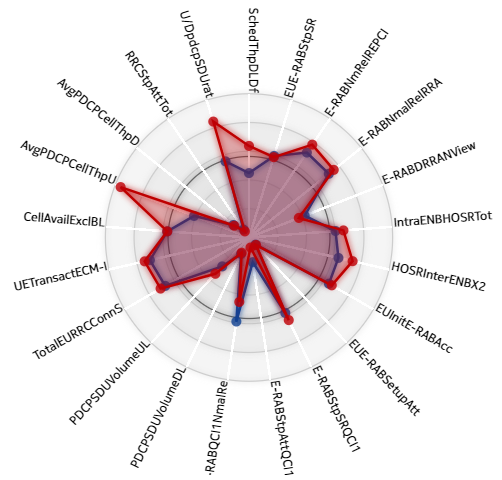
\includegraphics[width=0.4\linewidth]{figures/03_quantization/anomaly_pattern/anomaly_pattern.png}
				\caption[Anomaly pattern examples]{An example of an anomaly pattern (red) compared against the best match (blue) in the diagnosis knowledge base, depicted on a radar-chart.}
				\label{fig:anomaly_pattern}
			\end{figure}
			
			An anomaly detection function defines distinct \textbf{anomaly events} both temporally and spatially, by specifying the timeframe and the affected network elements of the anomaly.
			Using a larger scope of collected \ac{PM} measurements during the anomaly event, \textbf{anomaly patterns} are formed which describe the characteristics of the anomaly.
			The anomaly pattern can consist of a vector of the normalized anomaly levels of each \ac{KPI} in a cell or multiple cells, or the raw \ac{KPI} values during the anomaly.
			Often these values are aggregated over time in the anomaly pattern.		 	
			After an anomaly is detected and an anomaly pattern is established, a diagnosis component analyses the anomaly pattern and tries to determine its root cause.
					
			Like other semi-automated implementations of self-healing topics, diagnosis rules are often defined a-priori by an expert.
			This static rule-based diagnosis knowledge base goes against our goals of a fully-automated self-healing system.
			An alternative, which allows a more dynamic, automated collection and maintenance of the diagnosis knowledge base is to use \ac{CBR}, where the diagnosis of an anomaly event is done by automated generalization and extrapolation from previous, similar examples of anomalies.
			However, for \ac{CBR}-type diagnosis to work, preferably a large database of previously diagnosed anomalies would need to be maintained.
		
			Automated diagnosis is a complicated task, largely due to the less-constrained problem formulation, accentuated by the distributed and heterogeneous nature of mobile networks.
			As diverse as fault states can be, they occur only in very rare cases, which makes it near impossible to collect statistically meaningful data for each case.
			The lack of a statistically relevant amount of samples makes the reliable root-cause analysis extremely difficult, especially so when utilizing \ac{DL}, which mainly relies on plentiful training observations for a correct model formulation (see Sec.~\ref{cha:deep_learning:sec:overfitting}).
			Thus, it is of utmost importance that diagnosis information is collected and reused from every possible source, by sharing it between different contexts, such as different network deployments or timeframes, software versions, or other discontinuities that could otherwise invalidate the already learned models.
			
			The manual collection and maintenance of such a shared diagnosis knowledge base would be tedious and expensive at best.
			Therefore, automated knowledge sharing of insights is required to achieve a maintainable diagnosis system for self-healing.
			This would be especially important in cases, where new network functions are introduced in the network, or even completely new networks are deployed.
			Such cases where models are learned in one task and context, and are applied to another task or context, is called transfer learning.
			Typically, transfer learning is hard to achieve, and is currently one of the leading topics of research in machine learning.
		
		\subsection{Knowledge Sharing using Quantization}
		
			The goal of a diagnosis knowledge sharing process between autonomous and cognitive diagnosis functions in different contexts (e.g. in different network instances), is to be able to share insights in a way well-suited for \ac{CBR}-type diagnosis functions, and incrementally improve the diagnosis capabilities of each other.
			The scenario we discuss here is one where multiple \acp{LDA} are connected to a single \ac{CDA} (Fig.~\ref{fig:diag_lda_cda}).
			The \acp{LDA} manage local, context-specific diagnosis knowledge bases, which contain previously diagnosed anomaly patterns with their diagnosis attached as a label.
			The central \ac{CDA}'s goal is to collect, harmonize and retain a large base of diagnoses which contains the most prevalent anomaly patterns from all previously seen contexts.
			
			\begin{figure}[ht]
				\centering
				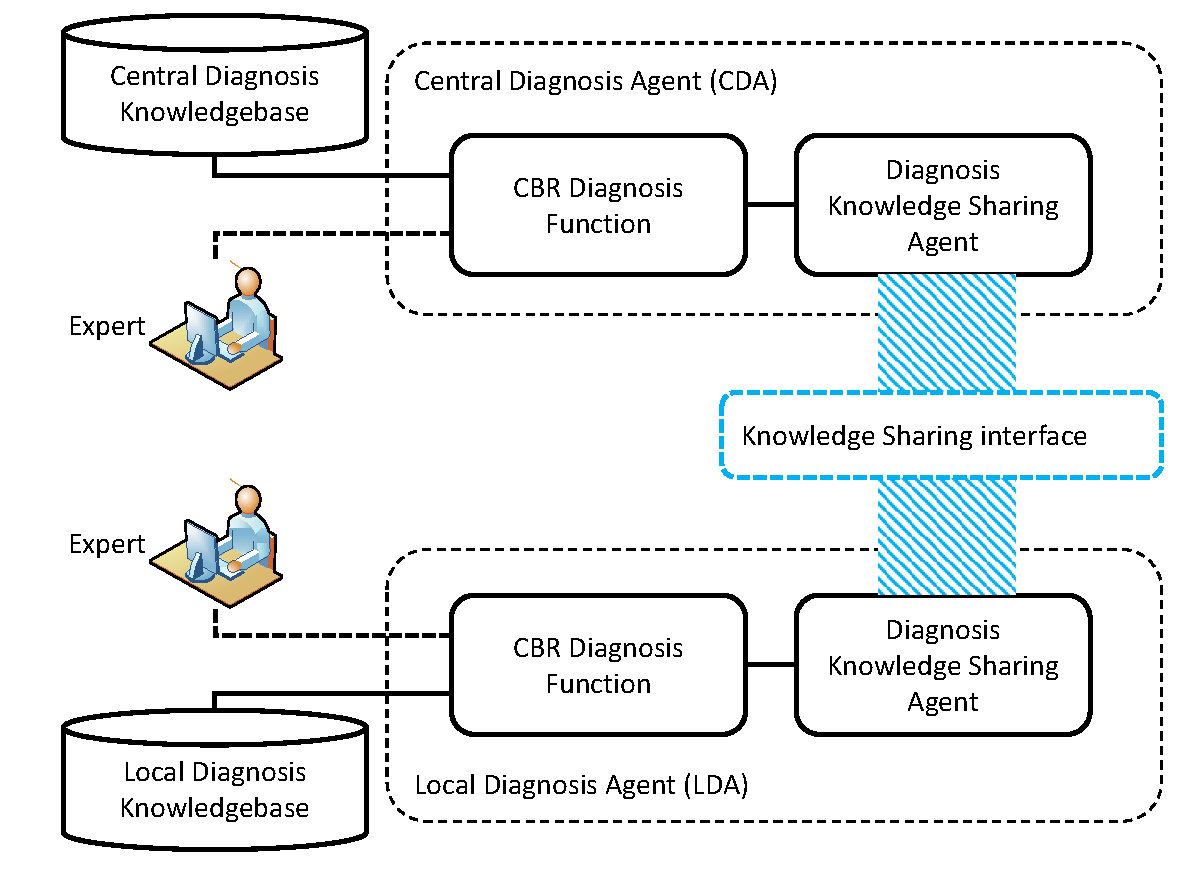
\includegraphics[width=0.8\linewidth]{figures/03_quantization/diag_lda_cda/diag_lda_cda.pdf}
				\caption[CBR diagnosis with knowledge sharing]{CBR diagnosis process with knowledge sharing.}
				\label{fig:diag_lda_cda}
			\end{figure}
			
			Both the local and central knowledge bases are updated either by a human expert, or a \ac{CBR}-type automated diagnosis function in case a new anomaly pattern is introduced.
			However, in order to realize knowledge sharing, the \acp{LDA} and the \ac{CDA} are connected through a \textit{knowledge sharing interface}.
			The communication on this knowledge sharing interface is imagined through the use of some form of vector quantization.
			
			The information communicated between the agents can be seen as a request for help in refining/extending their respective models.
			The information going in both directions is made up of labeled quanta, and optionally a collection of specific anomaly instances for which the respective agent decided that they do not fit its subjective model well.			
			Most quantization algorithms expect their input as a set of points, with a usual option of defining a starting position for the quantum centroid.
			However, here the quantization algorithms need to be able to run on an input comprised of a mix of clusters and outlying points.
			This functionality can be synthesized if individual points are sampled from a local database to recreate the distribution of points contained in the given clusters.
			If individual points were also communicated, these can be mixed to the synthesized points.
			Using this semi-synthetic set, the quantization algorithm can start from the locally saved previous state, and run until convergence.
			An example of the whole procedure can be seen in Fig.~\ref{fig:diag_knowledge_sharing}.			
			The (re-)sampling procedure allows the \ac{CDA} to maintain a diagnosis database of a constant size, rather than continuously collecting information.
			
			\begin{figure}[ht]
				\centering
				\subfloat[Input information]{
					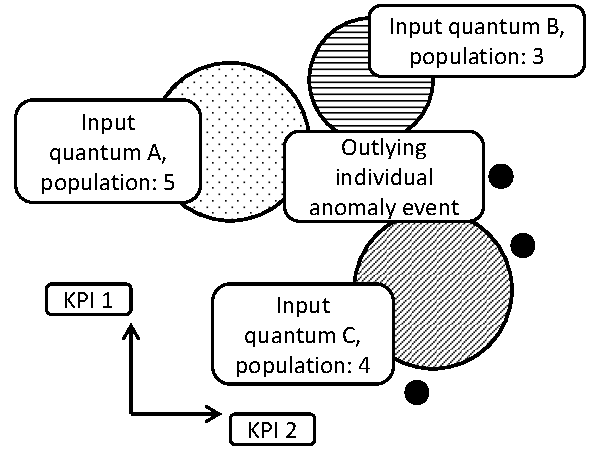
\includegraphics[width=0.4\linewidth]{figures/03_quantization/diag_knowledge_sharing/diag_knowledge_sharing_1.pdf}
				}
				\subfloat[Sampling and mixing]{
					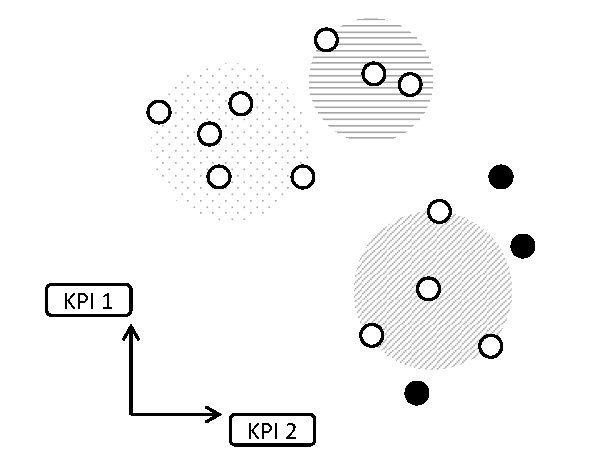
\includegraphics[width=0.4\linewidth]{figures/03_quantization/diag_knowledge_sharing/diag_knowledge_sharing_2.pdf}
				} \\
				\subfloat[Local model starting position]{
					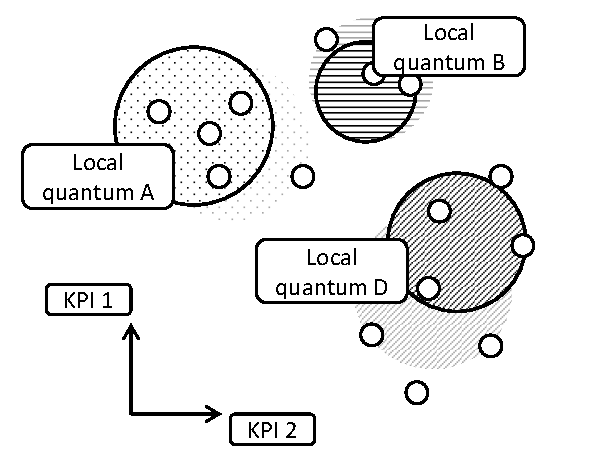
\includegraphics[width=0.4\linewidth]{figures/03_quantization/diag_knowledge_sharing/diag_knowledge_sharing_3.pdf}
				}
				\subfloat[fitting]{
					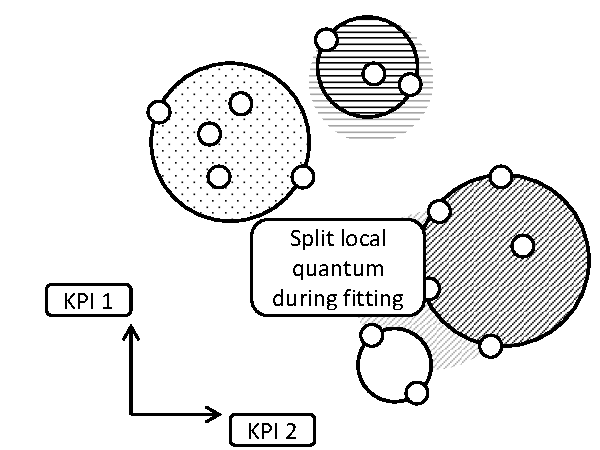
\includegraphics[width=0.4\linewidth]{figures/03_quantization/diag_knowledge_sharing/diag_knowledge_sharing_4.pdf}
				}
				\caption[Diagnosis knowledge sharing]{Quantization procedure incorporating local starting positions and mixed input information.}
				\label{fig:diag_knowledge_sharing}
			\end{figure}
			
			The quantization serves two purposes: firstly, it is a fine enough discretization of the anomaly pattern space, with which the different anomaly’s root causes can be described by attaching a single diagnosis/root cause to each of the quanta.
			Secondly, the quanta also serve to describe the anomaly event distribution in the anomaly pattern space, from which the original statistical distribution can be reconstructed/resampled with enough precision.			
			In the bigger picture, the described method transfers knowledge or new information from a source model to a target.
			This is true regardless of the source being the \ac{LDA} and the target being the \ac{CDA}, or vice-versa.
		
%		\subsection{Quantum Splitting and Merging}	
%			
%			To be able to automatically fit the model complexity to the complexity of the underlying data structure, quanta need to be dynamically added or removed from the model.
%			Automatic decisions can be implemented to decide when to split or merge quanta based on some form of goodness-of-fit value, which creates a measure of confidence in the model.
%			Model confidence should be higher if the goodness-of-fit increases, or if the model complexity decreases.
%			
%			\begin{figure}[ht]
%				\centering
%				\subfloat{
%					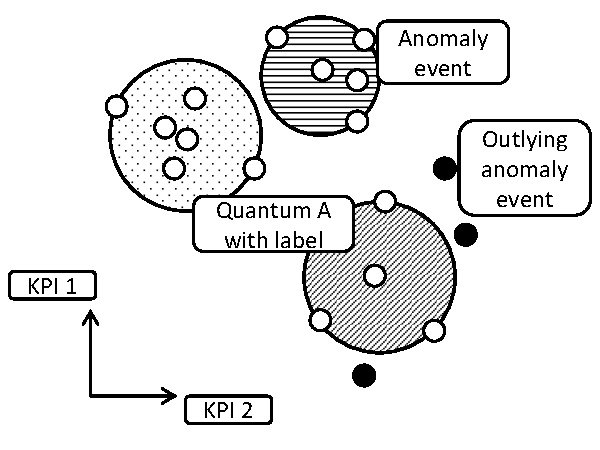
\includegraphics[width=0.4\linewidth]{figures/03_quantization/diag_split_merge/diag_split_1.pdf}
%				}
%				\subfloat{
%					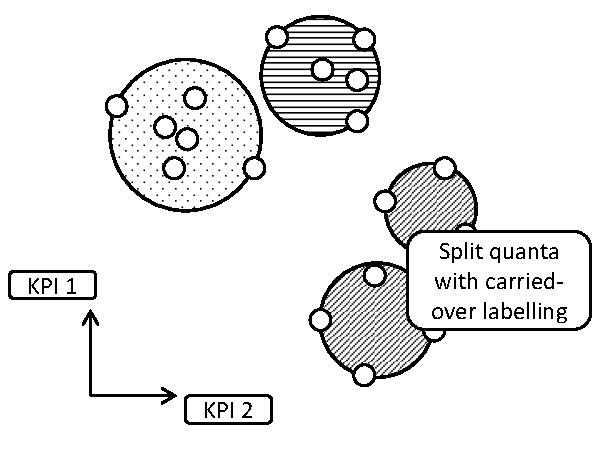
\includegraphics[width=0.4\linewidth]{figures/03_quantization/diag_split_merge/diag_split_2.pdf}
%				}
%				\caption{Quantum splitting.}
%				\label{fig:diag_split}
%			\end{figure}
%			
%			Splitting is done in case many points are lying outside a quantum, where an additional quantum could cover the outlying points so well that it counteracts the decrease in confidence stemming from the increased model complexity.
%			Split quanta should carry over labeling information within certain limits regarding distance from the original cluster, overlap of the clusters or surrounding clusters with the same/different labels.
%			If no labeling information can be assigned to the newly formed clusters with high confidence, clusters are left as unlabeled and the knowledge sharing process is started.
%			An example of cluster splitting can be seen in Fig.~\ref{fig:diag_split}.
%			
%			\begin{figure}[ht]
%				\centering
%				\subfloat{
%					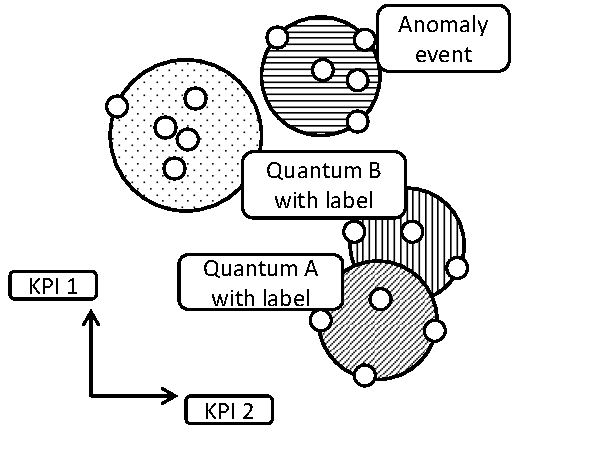
\includegraphics[width=0.4\linewidth]{figures/03_quantization/diag_split_merge/diag_merge_1.pdf}
%				}
%				\subfloat{
%					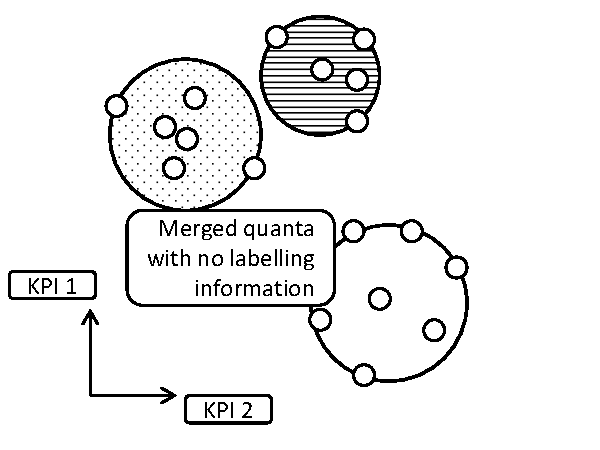
\includegraphics[width=0.4\linewidth]{figures/03_quantization/diag_split_merge/diag_merge_2.pdf}
%				}
%				\caption{Quantum merging.}
%				\label{fig:diag_merge}
%			\end{figure}
%			
%			The merging of quanta follows the same basic concept as splitting.
%			Two quanta should be merged if the decrease in model complexity overtakes the potential increase in goodness-of-fit.
%			Labeling information can be carried over from the original quanta if it fulfills criteria regarding similarity of parent labels, surrounding labels, and overlap.
%			Otherwise, the newly formed quantum is unlabeled and the knowledge sharing process is started.
%			An example of quanta merging can be seen in Fig.~\ref{fig:diag_merge}.

		% ITT - READ END

		\subsection{Towards Equal-Volume Quantization}
		
			The diagnosis knowledge sharing concept was the first occurrence in our work, where some form of quantization was meant to be used as a basis for communication between cognitive functions.
			Several aspects in it influenced the design of the bounding volume quantization algorithms, which are the topic of the next section (Sec.~\ref{cha:quantization:sec:bvq}):
			\begin{itemize}
				\item 
					\textbf{Equal volumes}:
					The roughly equal volumes of the quanta are needed to be able to establish a uniform ``resolution'', with which the labeling process operates.
					While providing a very simple goodness-of-fit metric (maximum quantization error), this also helps in the easy definition of cluster merging and splitting criteria based on relative distance between points and quantum centroids, or between two quantum centroids.
				
				\item
					\textbf{Continuous learning}:
					The knowledge sharing concept is built around a quantization, where the fitting procedure can be continued at any time, even if the training points are completely replaced.
					The \ac{EM} iterative optimization framework makes this inherently possible, by simply continuing the iterations whenever further fitting is required.
				
				\item
					\textbf{Mixed inputs}:
					The quantization algorithm was meant to be capable of fitting a mixed set of predefined quanta and individual observations without the proposed resampling mechanism.
					Although we did not propose this modification neither in the paper, nor in the invention, such a functionality was planned in case the knowledge sharing concept was to be further pursued.					
			\end{itemize}
			
			The diagnosis knowledge sharing concept was, in my opinion, quite far in the development process, close to being evaluated on data from a real mobile network deployment.
			Unfortunately, this data would have originated from an operator, with which Nokia ultimately could not agree on data-sharing conditions.
			Given this larger dataset, the work detailed in the next section would have also contained the evaluation results from the knowledge sharing scenario.
			Ultimately, lacking this dataset meant that we had to use a simpler, smaller dataset, which lead to us using use cases such as visualization or anomaly detection.
			In the end, we were never able to source large-scale network data of the type needed for this evaluation, thus the diagnosis knowledge sharing concept is only discussed in the respective patent.
	
	\section{Density-Invariant Quantization with Bounding Volumes}
		\label{cha:quantization:sec:bvq}
	
		\subsection{Quantization in High-Dimensional Spaces}
			\label{cha:quantization:sec:high_dim_problem}		
			
			Most often, quantization is used to refer to basic numerical processes, such as rounding to the nearest integer.
			While technically a correct interpretation, rounding and other per-dimension quantization methods are not feasible if the input data is high-dimensional.
			To illustrate this lack of scaling with the dimensionality, let us imagine a simple unit rectangle, populated by a number of points, representing the observations in our training dataset.
			The simplest quantization in this rectangle is to split every dimension into $2$ partitions, arriving at $4$ bins into which the datapoints can fall.
			By increasing the number of dimensions to $3$, the same scheme gives us $8$ bins, and so on.
			The equation (Eq.~\ref{eq:bin_curse_of_dim}) that governs the number of bins can be seen in Fig.~\ref{fig:perdim_curse}, where $n_{bins}$ refers to the number of attained bins, $p$ is the number of partitions per-dimension, and $d$ is the number of dimensions.
				
			\begin{figure}[ht]
				\centering
				\begin{minipage}[t]{0.2\linewidth}
					\begin{equation}
						\label{eq:bin_curse_of_dim}
						n_{bins} = p^d,
					\end{equation}
				\end{minipage}
				\begin{minipage}[t]{0.6\linewidth}
					\raisebox{-0.8\height}{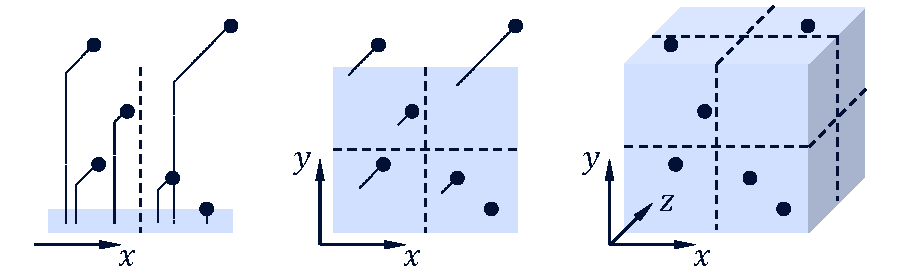
\includegraphics[width=\linewidth]{figures/03_quantization/perdim_quant/perdim_quant.pdf}}
				\end{minipage}
				\caption[Illustration of the curse of dimensionality in per-dimension quantization]{Illustration of the curse of dimensionality in per-dimension quantization.}
				\label{fig:perdim_curse}
			\end{figure}
			
			Increasing the dimensions further can quickly lead to a number of bins which is greater than the number of datapoints.
			This situation defeats the purpose of quantization; it is likely that some bins will be left unpopulated or contain only a few datapoints, while a few bins will contain the majority the datapoints.
			This situations means the quantization does not compress information effectively, or at all.
			It is easy to see that the exponential scaling of the number of bins with the number of dimensions can overcome any reasonably-sized dataset with even the lowest number of bins per dimension, thus, such quantization methods do not work with high-dimensional input data.
			This effect is just one aspect of the \emphix{curse of dimensionality}{curse of dimensionality} -- the behavior of high-dimensional spaces -- which will come up often in this thesis \cite{curse_of_dim}.
			
			Mobile network data exhibits the above described problem; in \acp{OSS}, thousands of \acp{KPI} are collected on a minutely basis, where \acp{KPI} function as separate dimensions, making up a high-dimensional space in which observations exist as individual datapoints.
			To achieve a sensible quantization in such spaces, instead of per-dimension quantization, vector quantization algorithms are used.
			These algorithms define a number of quanta in a way which is independent of the number of dimensions, freeing the quantization from the curse of dimensionality at least a little.
			Furthermore, the quanta ``stick'' to populated areas of space, so that every quanta is almost guaranteed to be populated (as long as $n_{quanta} \leq n_{datapoints}$).		
			
			In the following, multi-dimensional observations making up a dataset will are referred to as either datapoints, or just simply points.
			A set of points belonging to the same partition are referred to as a \emphix{quantum}{quantum}.
			A quantum \emphix{centroid}{centroid} is a single point -- a prototype -- that represents (the most important characteristics of) the whole quantum.
			The quantum centroid is neither necessarily the geometric center of the set of points, nor one of the points.
			The distance between a quantum centroid and an observation assigned to that quantum is the \emphix{quantization error}{quantization error} of that observation.
			The distance measure is the Euclidean distance (or squared distance, the $L_2$ metric) if not stated otherwise.
			If an area of the input space is sparsely populated (i.e.: contains few or no datapoints), it simply referred to as \emphix{sparse}{sparse space}, or \emphix{dense}{dense space} if the contrary is true.
			
			Vector quantization algorithms were originally conceived for the purpose of data compression.
			By replacing each observation with its closest quantum centroid, stored or transmitted information can be greatly compressed at the cost of losing the information contained within the quantization error vector.
			In the following, a (non-exhaustive) list of currently popular algorithms, and a brief description of their optimization targets is presented:
			\begin{itemize}
				\item 
					\textbf{\kmeans{}:} More precisely Lloyd's algorithm \cite{lloyd} was originally conceived as a signal quantization method.
					The \kmeans{} algorithm partitions the data into \textit{k} quanta so that the sum of quantization errors on all observations is minimal.
					This results in an accurate quantization of dense areas but a less precise quantization of sparse areas, for which a fewer number of quanta is assigned.
				
				\item 
					\textbf{Self-Organizing Maps, Neural Gases:} These algorithms follow the competitive learning paradigm, in which each quantum is competing with the others for a ``right to respond to a given subset of inputs'' \cite{complearn}.
					In this approach, areas that are sparsely populated present a smaller reward and draw fewer quanta, resulting in similar behavior to \kmeans{}.
				
				\item
					\textbf{Sparse Autoencoders:} Autoencoders show similar behavior to quantization methods if activation sparsity is enforced in the encoding; nodes in the hidden layers are assigned to (distinct) parts of the input space \cite{ksparse}.
					Activation sparsity refers to a different concept as previously introduced, and is discussed in more detail later in Sec.~\ref{cha:sparse_clust:sec:act_sparse}.
					Since autoencoders optimize data compression by minimizing the loss of overall information, this also translates to having fewer nodes assigned to sparsely populated areas in the input space, resulting in greater compression and greater quantization error in those areas.
			\end{itemize}
			\noindent Although the optimization targets of the approaches presented above are different, they result in similar behavior: sparse areas of the input space are mapped with less precision, quanta assigned to these have a greater maximum quantization error.
			
			In many applications, sparse areas of the data are just as important -- or even more important -- as dense areas.
			In these cases, the representation of densely and sparsely populated areas with at least the same precision is desired.
			Thus, instead of minimizing the sum of quantization errors, we propose that it is better to strive for the minimization of the maximum quantization error in these cases.
			Tightly fitting a bounding shape, such as a sphere, to wrap the points in a quantum allows us to define an assigned volume of the quantum.
			The bounding shape's exact position and size is only governed by the points farthest from the quantum center; in this regard, the points with the largest quantization error are effectively setting the assigned volume of the quantum they are in.
			Equal and minimal maximum quantization error between quanta can be achieved by the equalization of this assigned volume, which is the main idea presented in this section.
		
		\subsection{Uses of Equal-Volume Quantization in Mobile Networks}
			\label{cha:quantization:sec:equal_probelm}
			
			Mobile network \ac{PM} data often contains a wide variety of information acquired from different parts and layers of the network.
			With time-wise aggregation, \ac{PM} data is usually made up of vectors of \acp{KPI} for each granularity period, with each \ac{KPI} representing the performance of one characteristic of the network.
			These \acp{KPI}, often collected in hundreds for each granularity period, can be viewed as features or dimensions, with the \ac{PM} vectors selecting single points in a multi-dimensional space.
			Even after utilizing dimension reduction techniques such as \ac{PCA} on this data, the user is probably left with more than a handful of dimensions.
			Traditional tools, such as bar charts or 2D/3D scatter plots, can not efficiently visualize this information, and obfuscate underlying structure in the data.
			Quantization algorithms are often used in these cases for simplification (such as in \cite{laiho, kimmo}), with the resulting quanta viewed as usual \textit{types} of observations.
			The quanta then can be visualized effectively with bar charts, radar charts or heatmaps, by representing the whole area covered by a quantum with its centroid.
			An example of this can be seen in Fig.~\ref{fig:som}, where $6$ \acp{KPI} from mobile network \ac{PM} data were quantized with a \ac{SOM} consisting of $12$ units.
			
			\begin{figure}[ht]
				\centering
				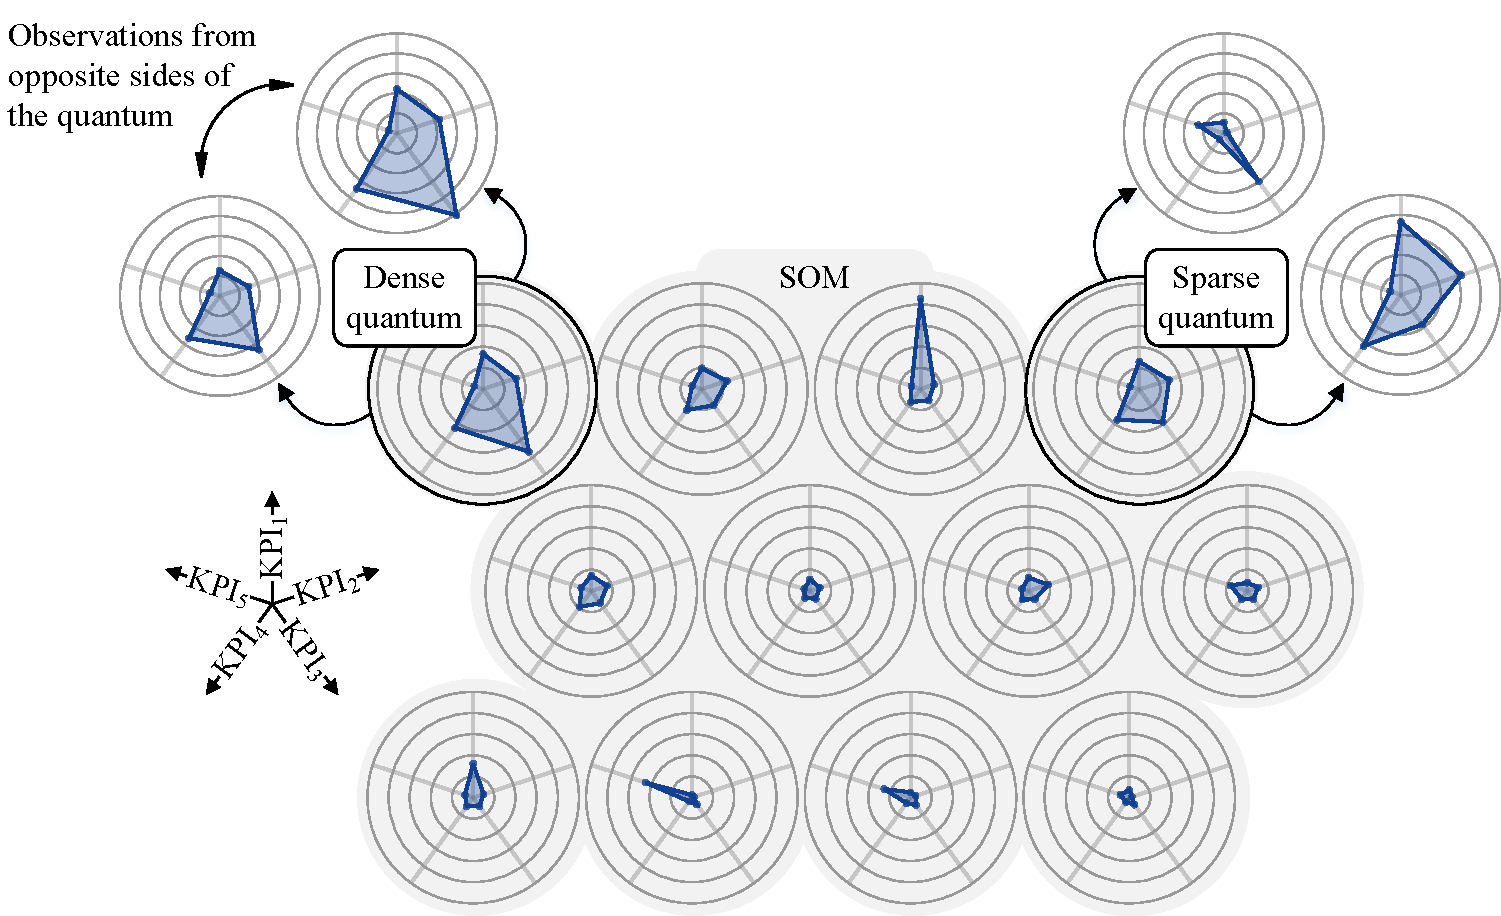
\includegraphics[width=\linewidth]{figures/03_quantization/som/som_pic.pdf}
				\caption[PM data exploration with a SOM]{Cylindrical, hexagonal-grid SOM fitted on PM data, the best-matching units (quantum centroids) plotted as radar charts.}
				\label{fig:som}
			\end{figure}
			
			A reasonable human expectation is that the plotted quanta are equal in some sense, which in the above example is neither true for span (volume), nor for number of points assigned.
			Figure~\ref{fig:som} highlights observations on opposite ends of both a densely and a sparsely populated quantum, to illustrate the different spans covered by these. 
			The difference is not intuitive, and could be overlooked by less experienced users.
			It is also worth noting that a lot of the quanta are close together (for example the middle row in Fig.~\ref{fig:som}), and in the case of this dataset, close to lower values.
			An example of this behavior can also be seen in Fig.~\ref{fig:kmeansanom} in the next section.
			Processing such data with traditional quantization techniques can create ``bland'' quanta that concentrate on these less interesting but densely populated areas, hiding a lot of the variety in the data.
			Equal-volume quantization could be of use here to create quanta with roughly even spans, which lends to easier understanding, and does not concentrate on densely populated areas.
			
			Another use case where equal-volume quantization could be useful are tasks focused on processing anomalous observations, such as in \cite{kumpulainen}.
			In mobile network management -- especially in \ac{SON} -- anomaly detection and diagnosis is a major research area, part of a larger-scale automation scheme called self-sealing.
			As self-healing requires human-like reasoning, machine learning is applied here to make autonomous functions smarter.
			In anomaly diagnosis use cases, the emphasis is on separating and categorizing anomalous observations, which are by definition rare occurrences.
			This means that anomalous observations usually inhibit sparsely populated areas in the input space.
			Applying conventional quantization techniques in these cases can remove too much information from anomalous observations, making separation or categorization of anomalies impossible.
			
			\begin{figure}[ht]
				\centering
				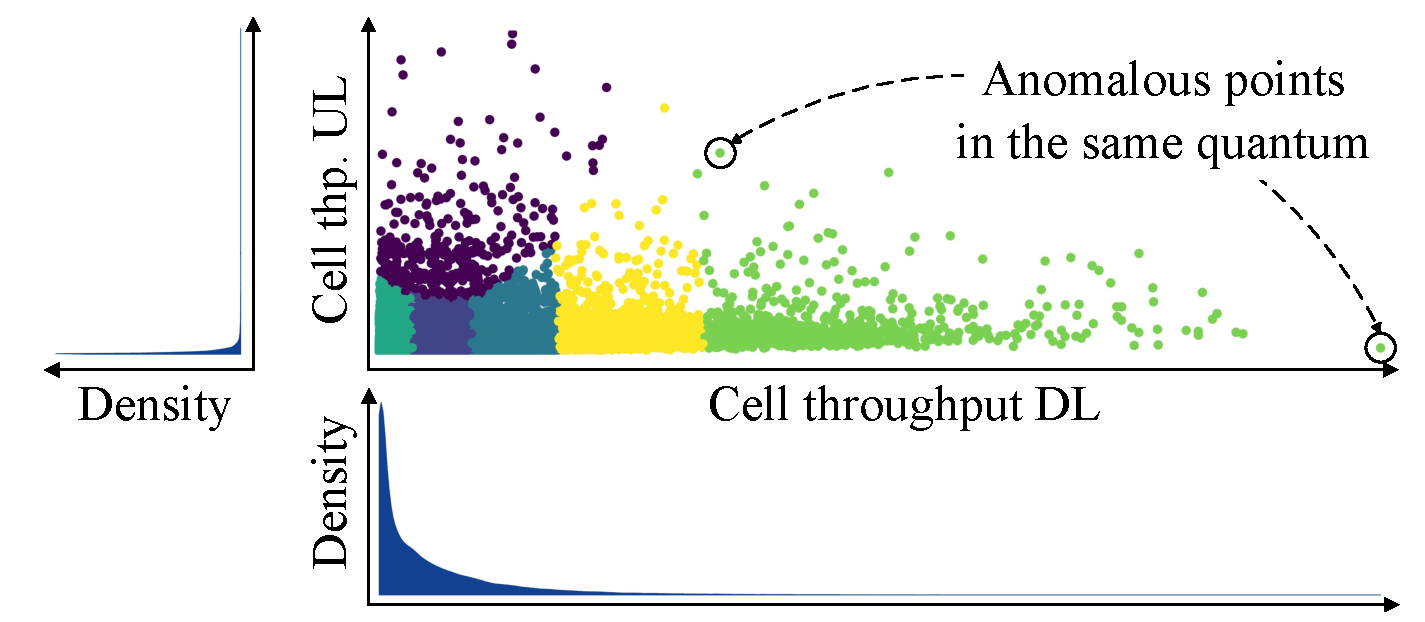
\includegraphics[width=0.8\linewidth]{figures/03_quantization/pm_kmeans_anom/pm_kmeans_anom.pdf}
				\caption[\kmeans{} quantization on PM data]{$2$ dimensions of PM data quantized with the \kmeans{} algorithm, showing obfuscated anomalous points.}
				\label{fig:kmeansanom}
			\end{figure}
			
			Figure~\ref{fig:kmeansanom} shows an example of this problem on $2$ \acp{KPI} taken from mobile network \ac{PM} data.
			The marginal densities show that most of the observations lie close to the origin ($0$ in all dimensions).
			Observations that lie further away from the origin are assigned to wider-spanning quanta, which makes it hard to differentiate between them, even if there are large actual distances between the points.
			Equal-volume quantization would process both sparse and dense areas with the same maximum error, thereby not allowing such great distances to be covered by a single quantum.
			
		\subsection{Expectation-Maximization and \kmeans{}}
			
			The key idea presented here is a quantization technique that tries to realize equal-volume quanta, thereby minimizing the maximum quantization error.
			Since volume is measured by fitting a bounding shape around the points assigned to a quantum, the minimization of the maximum quantization error heavily depends on the type of the fitted bounding shape.
			This work discusses quantization algorithms that utilize two types of bounding shapes: the sphere in case of \ac{BSQ}, and the axis-aligned box in case of \ac{BBQ}.
			Both algorithms are similar in algorithmic structure to Lloyd's \emphix{\kmeans{}}{k-means} algorithm.
			
			The global (across all quanta) optimization target of \kmeans{} is to partition a point set into $k$ quanta, so that the overall sum of all quantization errors is minimized.
			This also means that locally (in each quantum) centroids need to be in a position where the sum of distances between the centroid and all assigned observations is minimized.
			The global optimization problem is NP-hard for all but the simplest of cases \cite{kmeanscomp}, and as such exhaustive search makes little sense in real-life applications.
			The \kmeans{} algorithm solves this problem with the \emphix{\ac{EM}}{expectation-maximization} algorithmic structure \cite{em}, realizing an iterative optimization, where the following two steps are alternated:
			\begin{enumerate}
				\item \textbf{Expectation (assignment):} In this step all observations are assigned to one of the quanta, by choosing the closest lying quantum centroid, also called \ac{1NN} classification.
				The distance is measured with the Euclidean distance. 
				\item \textbf{Maximization (update):} In this step the quantum centroids are moved to new locations, to better model the assigned points in step 1.
				In \kmeans{}, the centroids are moved to the mean of the assigned points, which ensures the smallest sum of quantization errors for that quantum, and takes care of the local optimization target.
			\end{enumerate}
			
			\ac{EM} realizes an iterative optimization, which by its nature can only find local optimum solutions, and may continue for many iterations before converging. However, in practice \kmeans{} shows the following qualities that make it one of the most widely applied quantization algorithms:
			\begin{itemize}
				\item The runtime of the algorithm is usually short even for large number of points, quanta or dimensions.
				\item It uses the Euclidean distance which is intuitive and easy to visualize.
				\item The solutions are close to optimal in most cases.
			\end{itemize}
			\noindent The short perceived runtime is a result of the relatively simple computations required by the algorithm, which, combined with the Euclidean distance, also makes it easy to understand.
			Although the \ac{EM} structure realizes greedy optimization, it generally gives good overall results with a fast convergence \cite{lloydeffective}.
			In order to retain these qualities, \ac{BSQ} and \ac{BBQ} keeps the main aspects and the overall structure of \kmeans{}.
			
		\subsection{Bounding Sphere Quantization}
			
			The optimization target of \emphix{\ac{BSQ}}{bounding sphere quantization} is to have minimal maximum quantization error both within each quantum (local optimization target), and overall in the quantization (global optimization target).
			The local target means for each quantum to have the farthest lying points equidistant from the quantum center, i.e. on a surface of a hypersphere whose center is the quantum centroid.
			There is exactly one such hypersphere with the smallest achievable radius for any set of points, which is called the minimal bounding sphere (or smallest enclosing ball) \cite{sebdef}.
			
			\ac{BSQ} differs from \kmeans{} in the maximization step, where instead of relocating the quantum centroid to the mean of the assigned points, a minimal bounding sphere is fitted to the points, and the quantum centroid is moved to the center of the sphere.
			An example of this is shown in Fig.~\ref{fig:bsqmax}.
			
			\begin{figure}[ht]
				\centering
				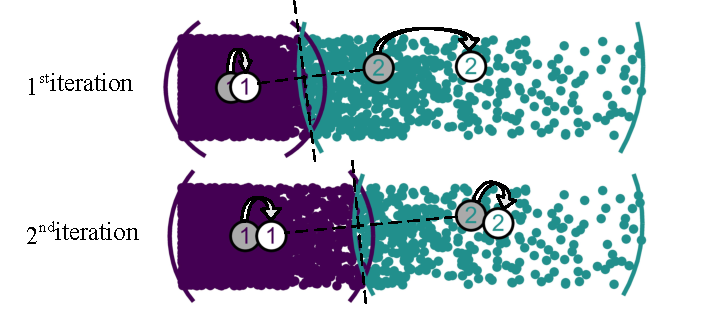
\includegraphics[width=0.7\linewidth]{figures/03_quantization/bsq_step/bsq_step.pdf}
				\caption[BSQ maximization step]{The maximization step of the BSQ algorithm.}
				\label{fig:bsqmax}
			\end{figure}
			
			The global optimization target is reached through the interplay between the \ac{1NN} classification in the expectation step, and the centering of the quantum centroids in the maximization step.
			\ac{1NN} assigns points to the closest centroid, which places the dividing line for assignment exactly halfway between centroids.
			By moving the quantum centroid to the center of the partition, the distance between neighboring quantum centroids tends to even out, producing quanta with equal radii. This tendency can also be observed in Fig.~\ref{fig:bsqmax}.
			Since radius is the only parameter that defines the volume of a sphere, this also translates to producing equal-volume quanta.
			
			We would like to emphasize the importance of data preprocessing -- in particular the normalization/standardization of dimensions -- as is usual for most machine learning methods.
			\ac{BSQ} considers each dimension on the same scale; dimensions that cover a greater span will contribute more to the quantization.
			For \ac{BSQ} to consider all dimensions with the same importance, dimensions need to be transformed to the same scale, or alternatively, importance can be set by the specific scaling of the dimensions.
			
			Stemming from the local nature of the \ac{EM} optimization, it is very important to initialize the algorithms correctly to be able to find solutions close to the global optimum and not get stuck in local optima.
			For the \kmeans{} algorithm, initialization is a well-researched subject with plenty of different approaches \cite{celebi_comparative}.
			The simplest way of initializing \kmeans{} is to randomly pick \textit{k} points from the point set as starting centroids.
			This makes sense for \kmeans{} as the the end goal is to have more quanta in denser areas.
			By randomly picking, it is more likely to pick from densely populated parts of the input space, thereby already approximating a good end result.
			
			In \ac{BSQ}'s case this is somewhat counter-productive, as random sampling produces starting quanta with uneven volumes.
			Picking actual points from the data as starting centroids does have a big benefit however: all quanta have at least one point assigned at all times.
			Since quanta naturally ``stick'' to points throughout the iterations, this means that a quantum can never lose all its assigned points, and the outcome of the quantization will always contain the preset \textit{k} number of quanta.
			If not actual points are picked, a misaligned initialization can produce a starting set where one or more of the quanta get ``pushed out'' of the populated areas of the input space, and lose all assigned points.
			A good candidate for \ac{BSQ}'s initialization is the greedy Farthest-First Traversal algorithm, that will be explained in more detail in Section \ref{cha:quantization:sec:related}.
			
			\ac{BSQ} has a clear stopping criterion; convergence is achieved when the assignment of points does not change for two consecutive iterations.
			As mentioned previously, \kmeans{} solves an NP-hard problem with the EM algorithmic structure.
			Although the usual runtime is short, \kmeans{} has a superpolynomial upper bound to the number of possible iterations in the worst case \cite{kmeansslow}.
			The same applies to \ac{BSQ}, but in this case complexity is further worsened by the maximization step; a minimal bounding sphere has to be fit on each quanta in each iteration separately.
			The algorithm of our choice for fitting the spheres is Fischer's exact solver \cite{fischer}, which is capable of finding the exact minimal bounding sphere of a large set of points in a basically arbitrary number of dimensions.
			Furthermore, Fischer's algorithm is also capable of fitting both spheres and points \cite{balls_of_balls} (points are in this sense spheres with $0$ radius), an important property in the context of diagnosis knowledge sharing.
			However, along with these good properties comes one drawback: Fischer's algorithm also realizes an iterative search, and unfortunately has no polynomial upper bound for the number of possible iteration steps. The two nested searches can in theory produce very long runtimes.
			
			As with all algorithms, runtime governs the usefulness of \ac{BSQ}, and can severely limit the possible use cases it can be applied to, so it is in our best interest to speed it up as much as possible.
			The three main parameters that set the overall complexity of the task are the number of points (\textit{n}), the number of dimensions (\textit{d}) and the number of quanta (\textit{q}).
			The \textit{n} and \textit{d} parameters represent the size of the input dataset, and in our experience can reach large values depending on the data source.
			The \textit{q} parameter represents the desired output, the simplified dataset, and so is not governed by the size of the input data, but rather by the use case itself.
			In the evaluated cases in this work, the number of quanta never exceeded more than a few hundred, thus our implementation \ac{BSQ} usually spent the majority (more than $60\%$) of time in the maximization step.
			Taking this into account, and in order not to break the \ac{EM} structure and the resemblance to \kmeans{}, the primary place where \ac{BSQ} could be sped up is at the fitting of minimal bounding spheres.
			
			There are many alternatives to Fischer's algorithm to fit minimal bounding spheres, of which a nice summary can be found in \cite{sebsum}.
			In the following is list of algorithms that were considered, and the reason they were ultimately discarded as a replacement:
			\begin{itemize}
				\item Solvers based on linear programming and designed for computational geometry in 3D, such as Megiddo's \cite{megiddo} or Welzl's \cite{welzl} algorithm, become inefficient already for moderately high dimensions, such as $\text{\textit{d}}>30$ \cite{fischer}.
				
				\item G\"{a}rtner and Sch\"{o}nherr's \cite{gartner} solver based on quadratic programming is polynomial in \textit{d}, but requires arbitrary-precision algebra that limits its use to $\text{\textit{d}}<300$ \cite{fischer}, which, although a relatively high number, would possibly exclude \ac{BSQ} from some of the use cases we considered.
				
				\item Zhou's algorithm \cite{zhou} is designed for very large values of \textit{d}, with the assumption that there are generally fewer points than dimensions, which is not applicable for our purposes.
				
				\item Kumar's approximating algorithm \cite{kumar} based on core-sets is outperformed by Fischer's algorithm with the latter also providing exact solutions \cite{fischer}.
				Furthermore, there exists a random sampling in the implementation of the algorithm which could also interfere with the stopping criterion, as it would make it hard to determine whether a change in assignment was made because of legitimate move of the centroids, or because of the dynamic error of this algorithm.
			\end{itemize}
			
			Relaxing the criteria of exact bounding sphere computation and allowing some error in the maximization step opens up more possible ways forward.
			Ritter's algorithm \cite{ritter}, a popular approximation used for computational geometry, usually fits bounding spheres $5-20\text{\%}$ larger than the smallest possible.
			Different from Kumar's approximation, here the error is static, so the outcome of subsequent runs on the same set of points does not change.
			The algorithm is very fast, but still realizes a few iterations of search.
			Because its complexity scales linearly with both \textit{d} and \textit{n}, it would be a good choice for speeding up \ac{BSQ}, even with the considerable approximation error. 
			
			Another possibility is to use a simpler shape as bounding volume.
			The simplest bounding shape to compute is the axis-aligned bounding box, which is the topic of the next section.
			
		\subsection{Bounding Box Quantization}
			
			\ac{BBQ} approximates the results of \ac{BSQ} by fitting axis-aligned bounding boxes on quanta instead of spheres.
			This can be done in a single pass on the whole dataset, by finding the maximum and minimum values of each dimension for each quanta.
			The quantum centroids are then moved to the center points of the bounding boxes in the maximization step.
			As such, the computational complexity of the maximization step is linearly dependent on both \textit{n} and \textit{d}, bringing the overall computational complexity of \ac{BBQ} back in line with that of \kmeans{}.
			
			Bounding boxes are theoretically bad approximations of bounding spheres.
			This is not apparent at first glance, as the Euclidean distance between the center points of the minimal bounding sphere and the minimal bounding box -- from now on referred to as \emphnox{approximation error} -- fitted on the same group of points is comparatively low in $2$ and $3$ dimensions, even in the worst cases.
			However, this theoretical threshold can be increased beyond any limit by adding enough dimensions, even if the error is measured relative to the bounding sphere radius (\textit{R}). Constructing point sets that create the largest approximation error (worst-sets) is possible for any \textit{d} following the logic in Fig.~\ref{fig:boxworstsets}.
			It is interesting to note that in $5$ dimensions or more, the center of the bounding box can actually be outside of the bounding sphere.
			The equation for the theoretical maximum approximation error is as follows:
			\begin{equation}
				|e_{\text{approx}_{\text{max}}}| = \sqrt{\frac{1}{4}(d-1)} R.
			\end{equation}
			
			\begin{figure}[ht]
				\centering
				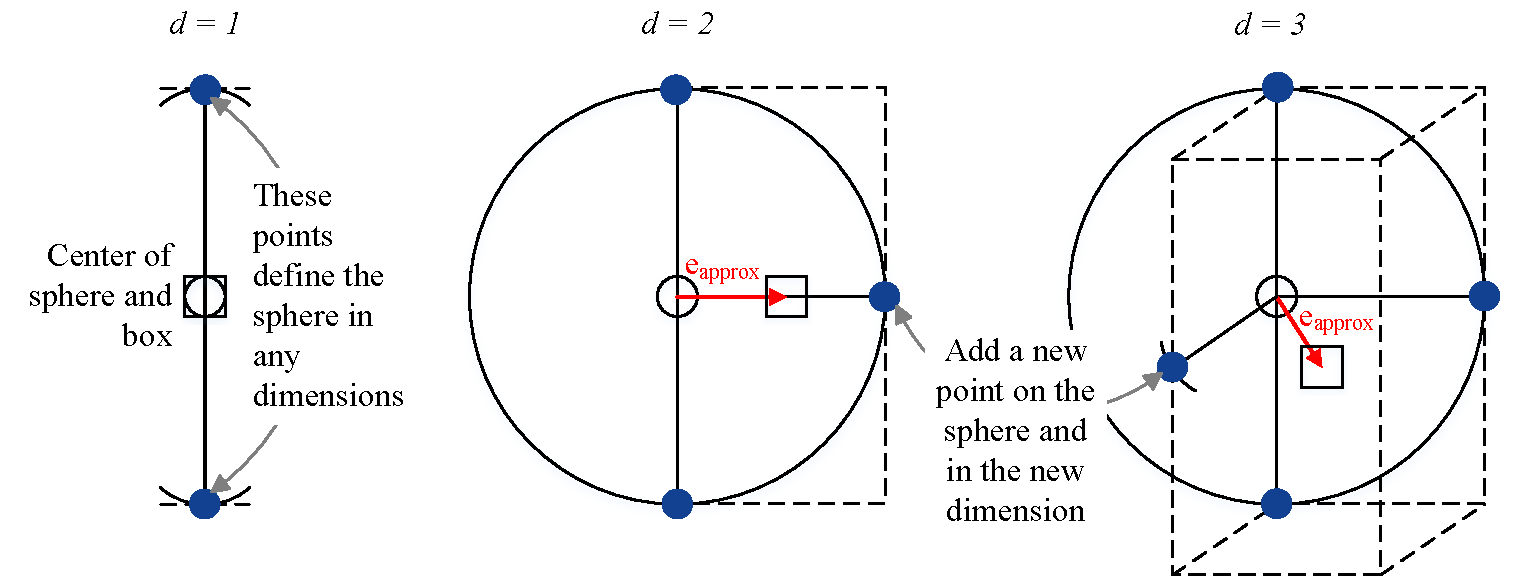
\includegraphics[width=\linewidth]{figures/03_quantization/worst_sets/worst_sets.pdf}
				\caption[BBQ worst-set construction]{Construction of worst-sets for maximum approximation error.}
				\label{fig:boxworstsets}
			\end{figure}
			
			Fortunately, in practice, bounding boxes are not as bad approximators as the theoretical limits show.
			While the maximum possible error increases in higher dimensions, the probability of a worst (or close to worst) set occurring decreases rapidly.
			This makes the expected approximation error in practice much smaller than the theoretical maximum.
			Measurements run for a single group of points for a wide range of \textit{n} and \textit{d} can be seen in Fig.~\ref{fig:boxrealsets}.
			For each combination of \textit{n} and \textit{d}, $10000$ random set of points were generated using a normal distribution with $0$ mean and a variance of $1$, independently for each dimension.
			After this, both a minimal bounding sphere and a minimal bounding box were fitted on each set, and the distance of the centroids measured.
			The experiment was also undertaken for data with a uniform distribution, but do not show these here as they produced almost identical results.
			
			\begin{figure}[ht]
				\centering
				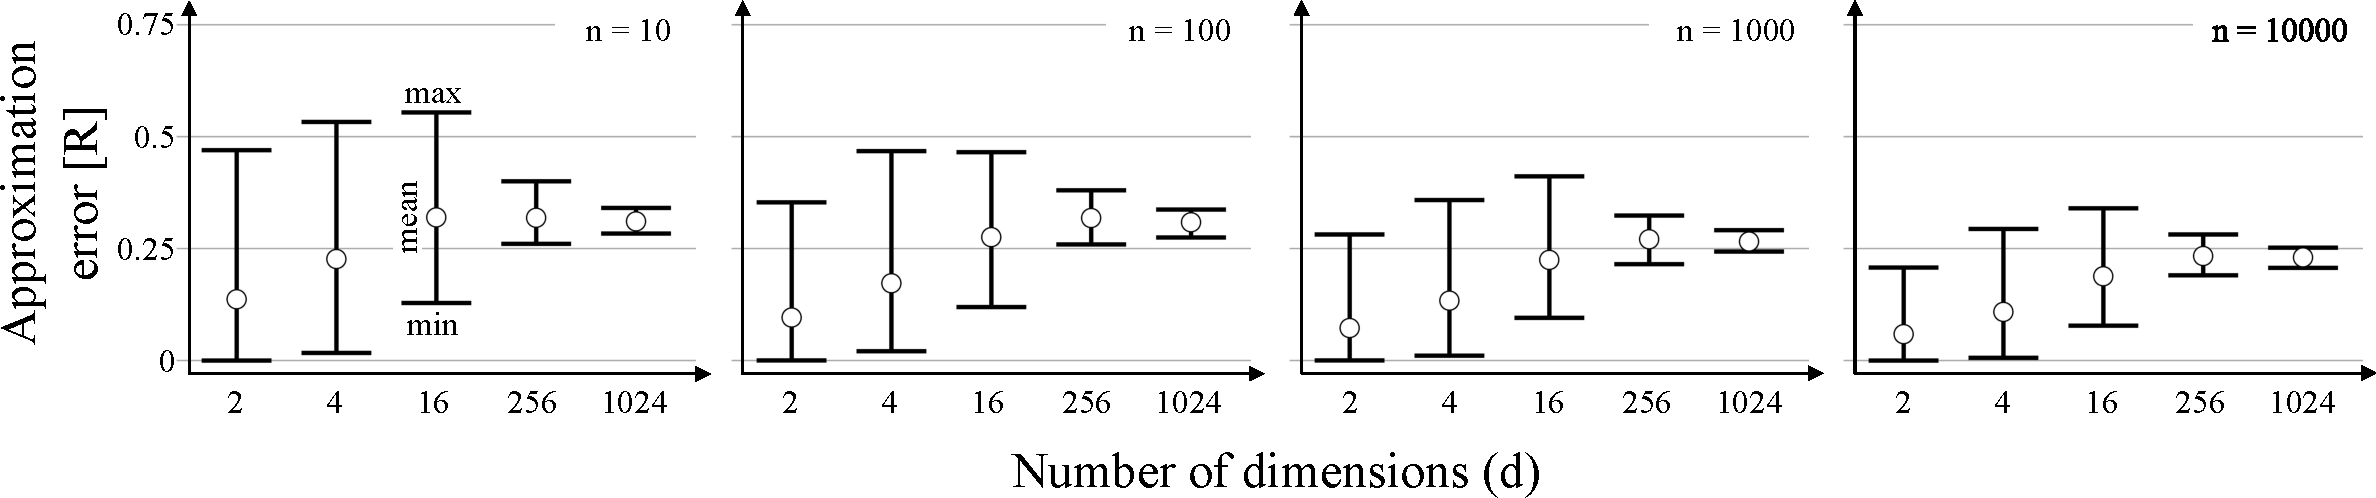
\includegraphics[width=\linewidth]{figures/03_quantization/error_whisk/error_whisk.pdf}
				\caption[BBQ approximation error distribution]{Distribution of approximation error (measured in the fitted minimal bounding sphere radius, $R$, fitted on $n$ randomly sampled points from a Gaussian).}
				\label{fig:boxrealsets}
			\end{figure}
			
			The decreased probability of worst-sets occurring seemed to counteract the larger possible error, so that the average approximation error never exceeded $0.33 R$, and the maximum $0.55 R$ in any of the generated sets.
			Increasing either \textit{d} or \textit{n} always seemed to lower the expected error, so that high \textit{d} but low \textit{n} values (sparse sets) also did not produce larger approximation errors.
			Interestingly, by increasing \textit{d}, the minimum error also increased, creating very narrow windows for expected error in high \textit{d}.
			Based on this, boxes appear to be are good approximators for bounding spheres if the data behaves nicely, i.e., has a continuous distribution that does not generate groups resembling worst sets.
			Such badly behaving data could be where all dimensions can only take a few fixed values, such as integer-rounded \acp{KPI} in small ranges (only a few tens).
			
			Minimal bounding boxes actually minimize the maximum dimension-wise distance between the points in the quantum and the centroid, essentially realizing the same functioning as minimal bounding spheres, but with the $L_\infty$ distance metric.
			This view explains why running \ac{BBQ} with the original \ac{1NN} assignment step utilizing the Euclidean distance causes the algorithm to not converge in higher dimensions.
			By using two different distance metrics, the assignment and update steps do not optimize for the same target, and move the quantization in different directions.
			This dissonance can be alleviated by changing the distance metric to the $L_\infty$ in the \ac{1NN} classification.
			In this case, points are assigned to the quantum centroid from which the largest dimension-wise distance is minimal.
			This modification essentially makes \ac{BBQ} the equivalent of \ac{BSQ} in a space where distance is measured with the $L_\infty$ metric.
			An example outcome of \ac{BSQ} and \ac{BBQ} starting from the same positions on 2-dimensional artificial data can be seen in Fig.~\ref{fig:bsqbbqexample}.
	
			\begin{figure}[ht]
				\centering
				\subfloat[BSQ]{
					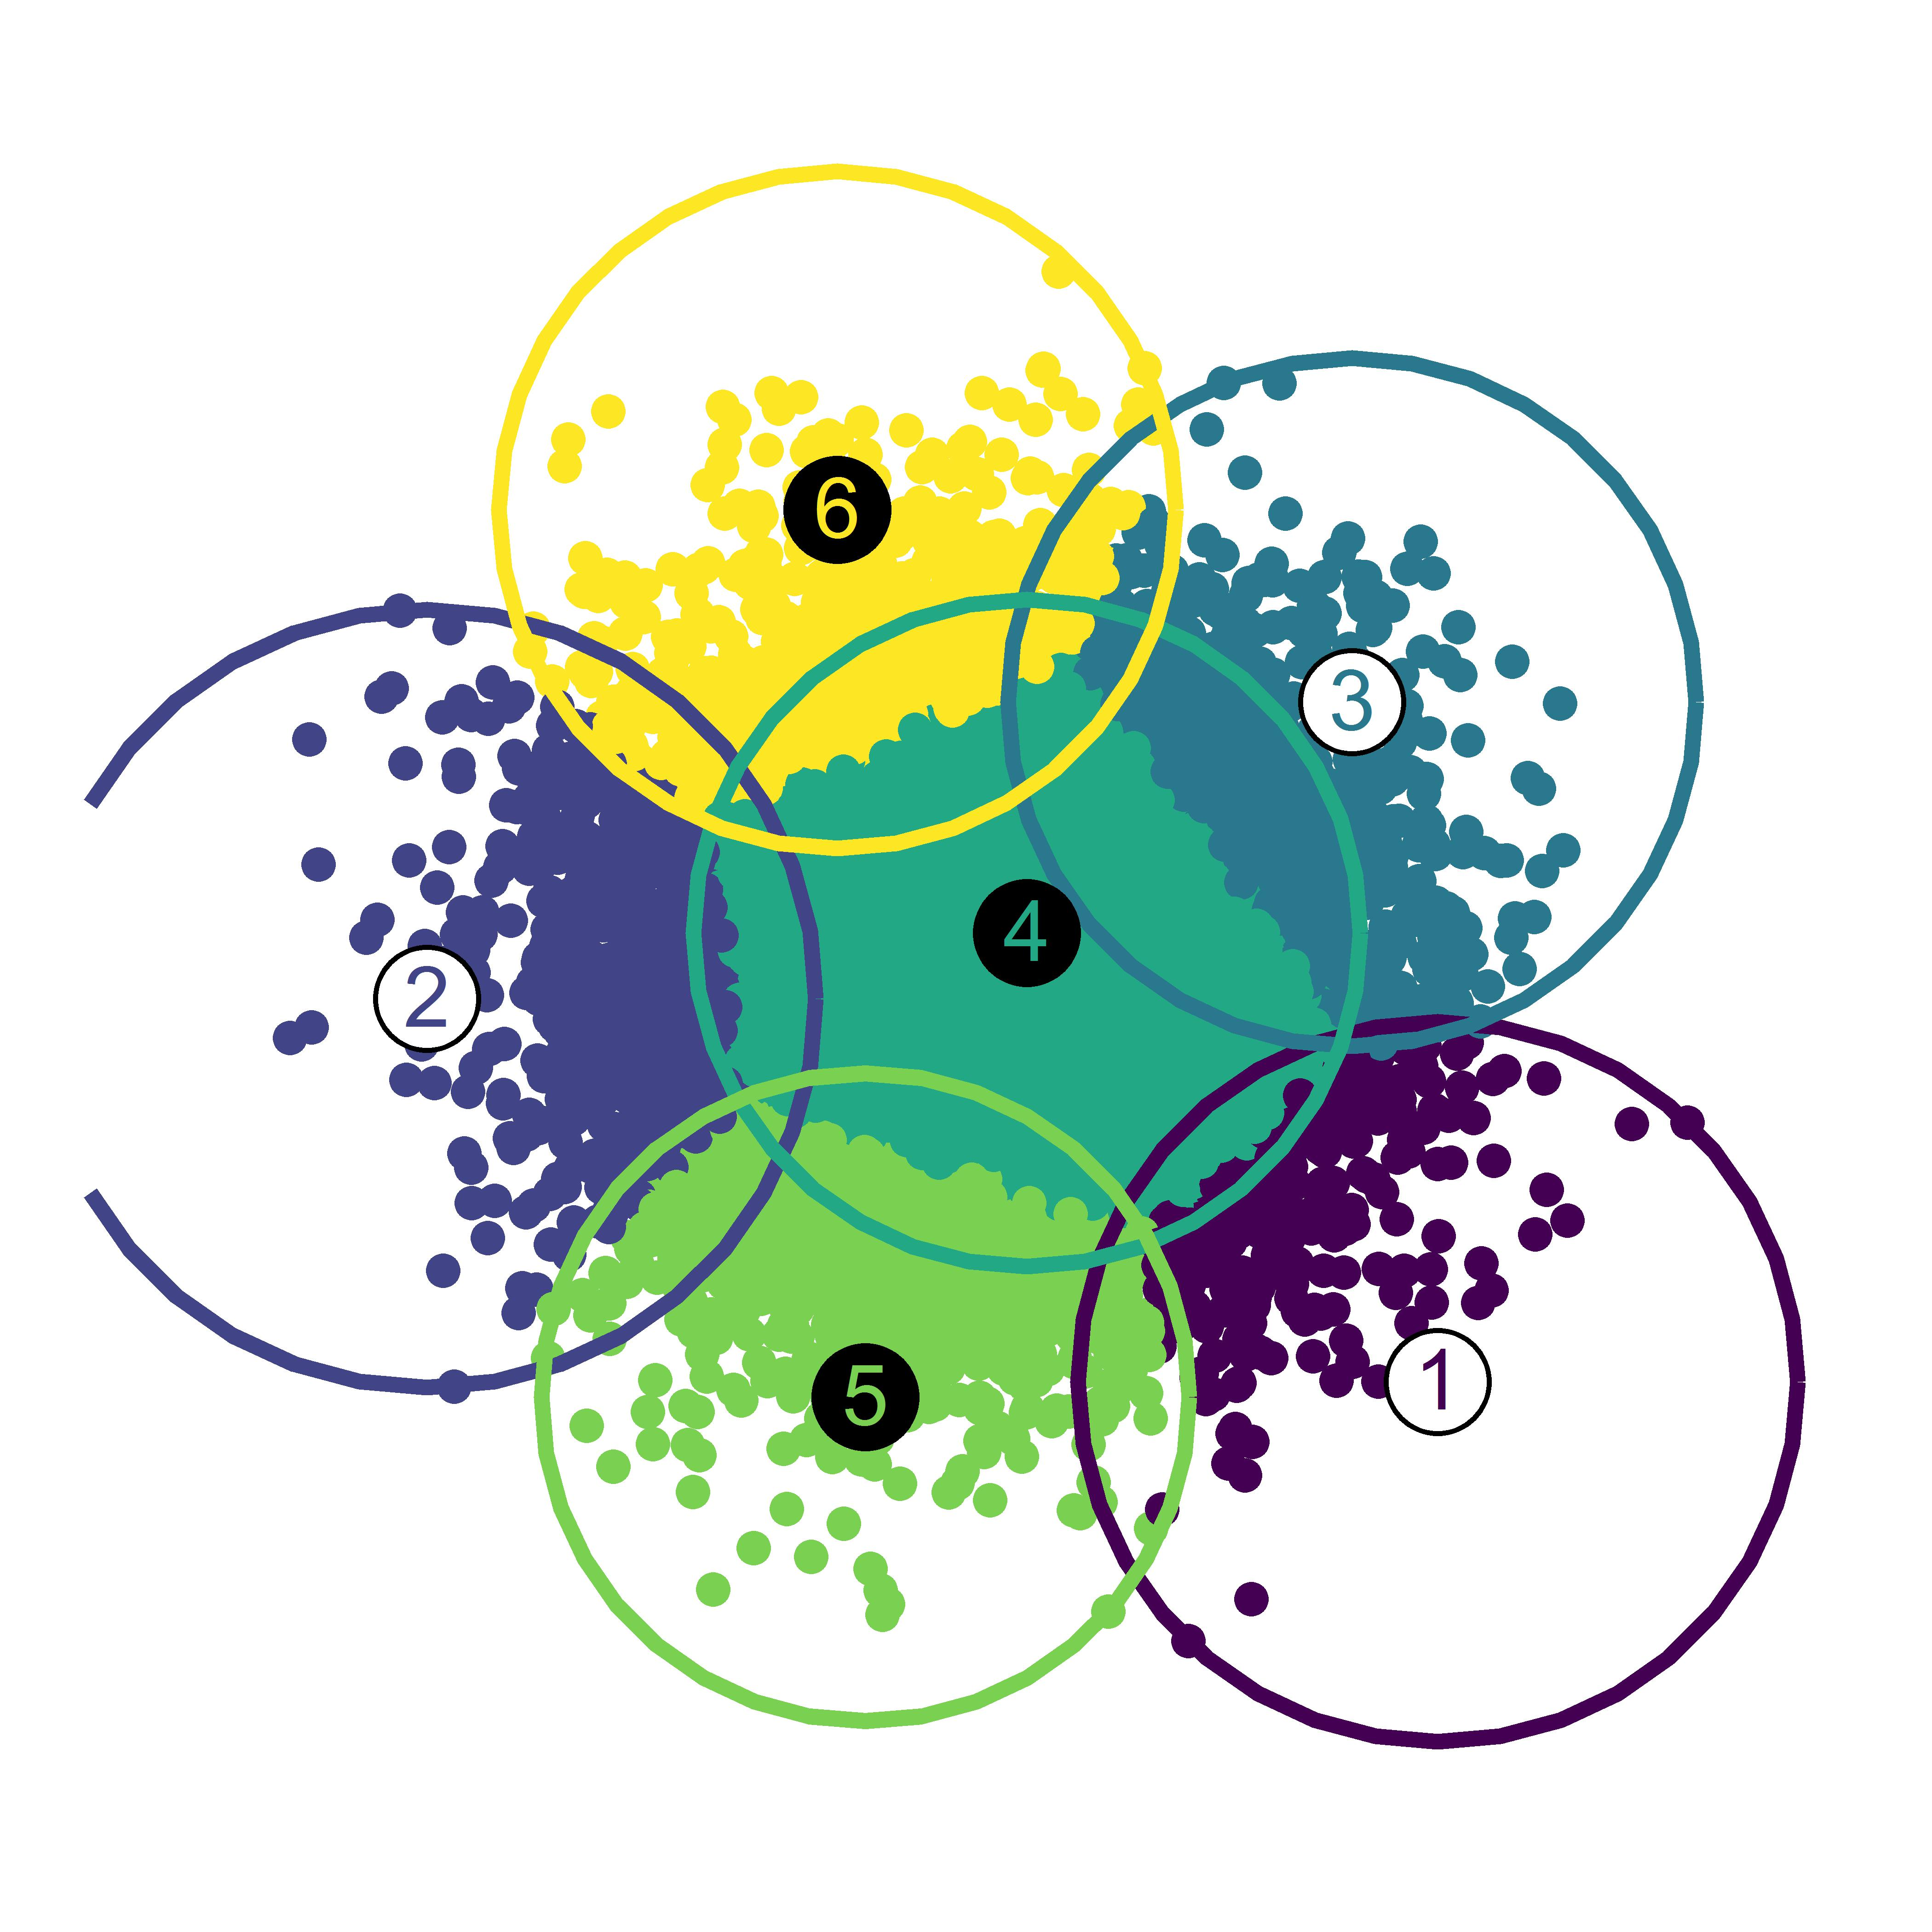
\includegraphics[width=0.4\linewidth]{figures/03_quantization/bsq_bbq_scatter/bsq_scatter.jpeg}
				}
				\subfloat[BBQ]{
					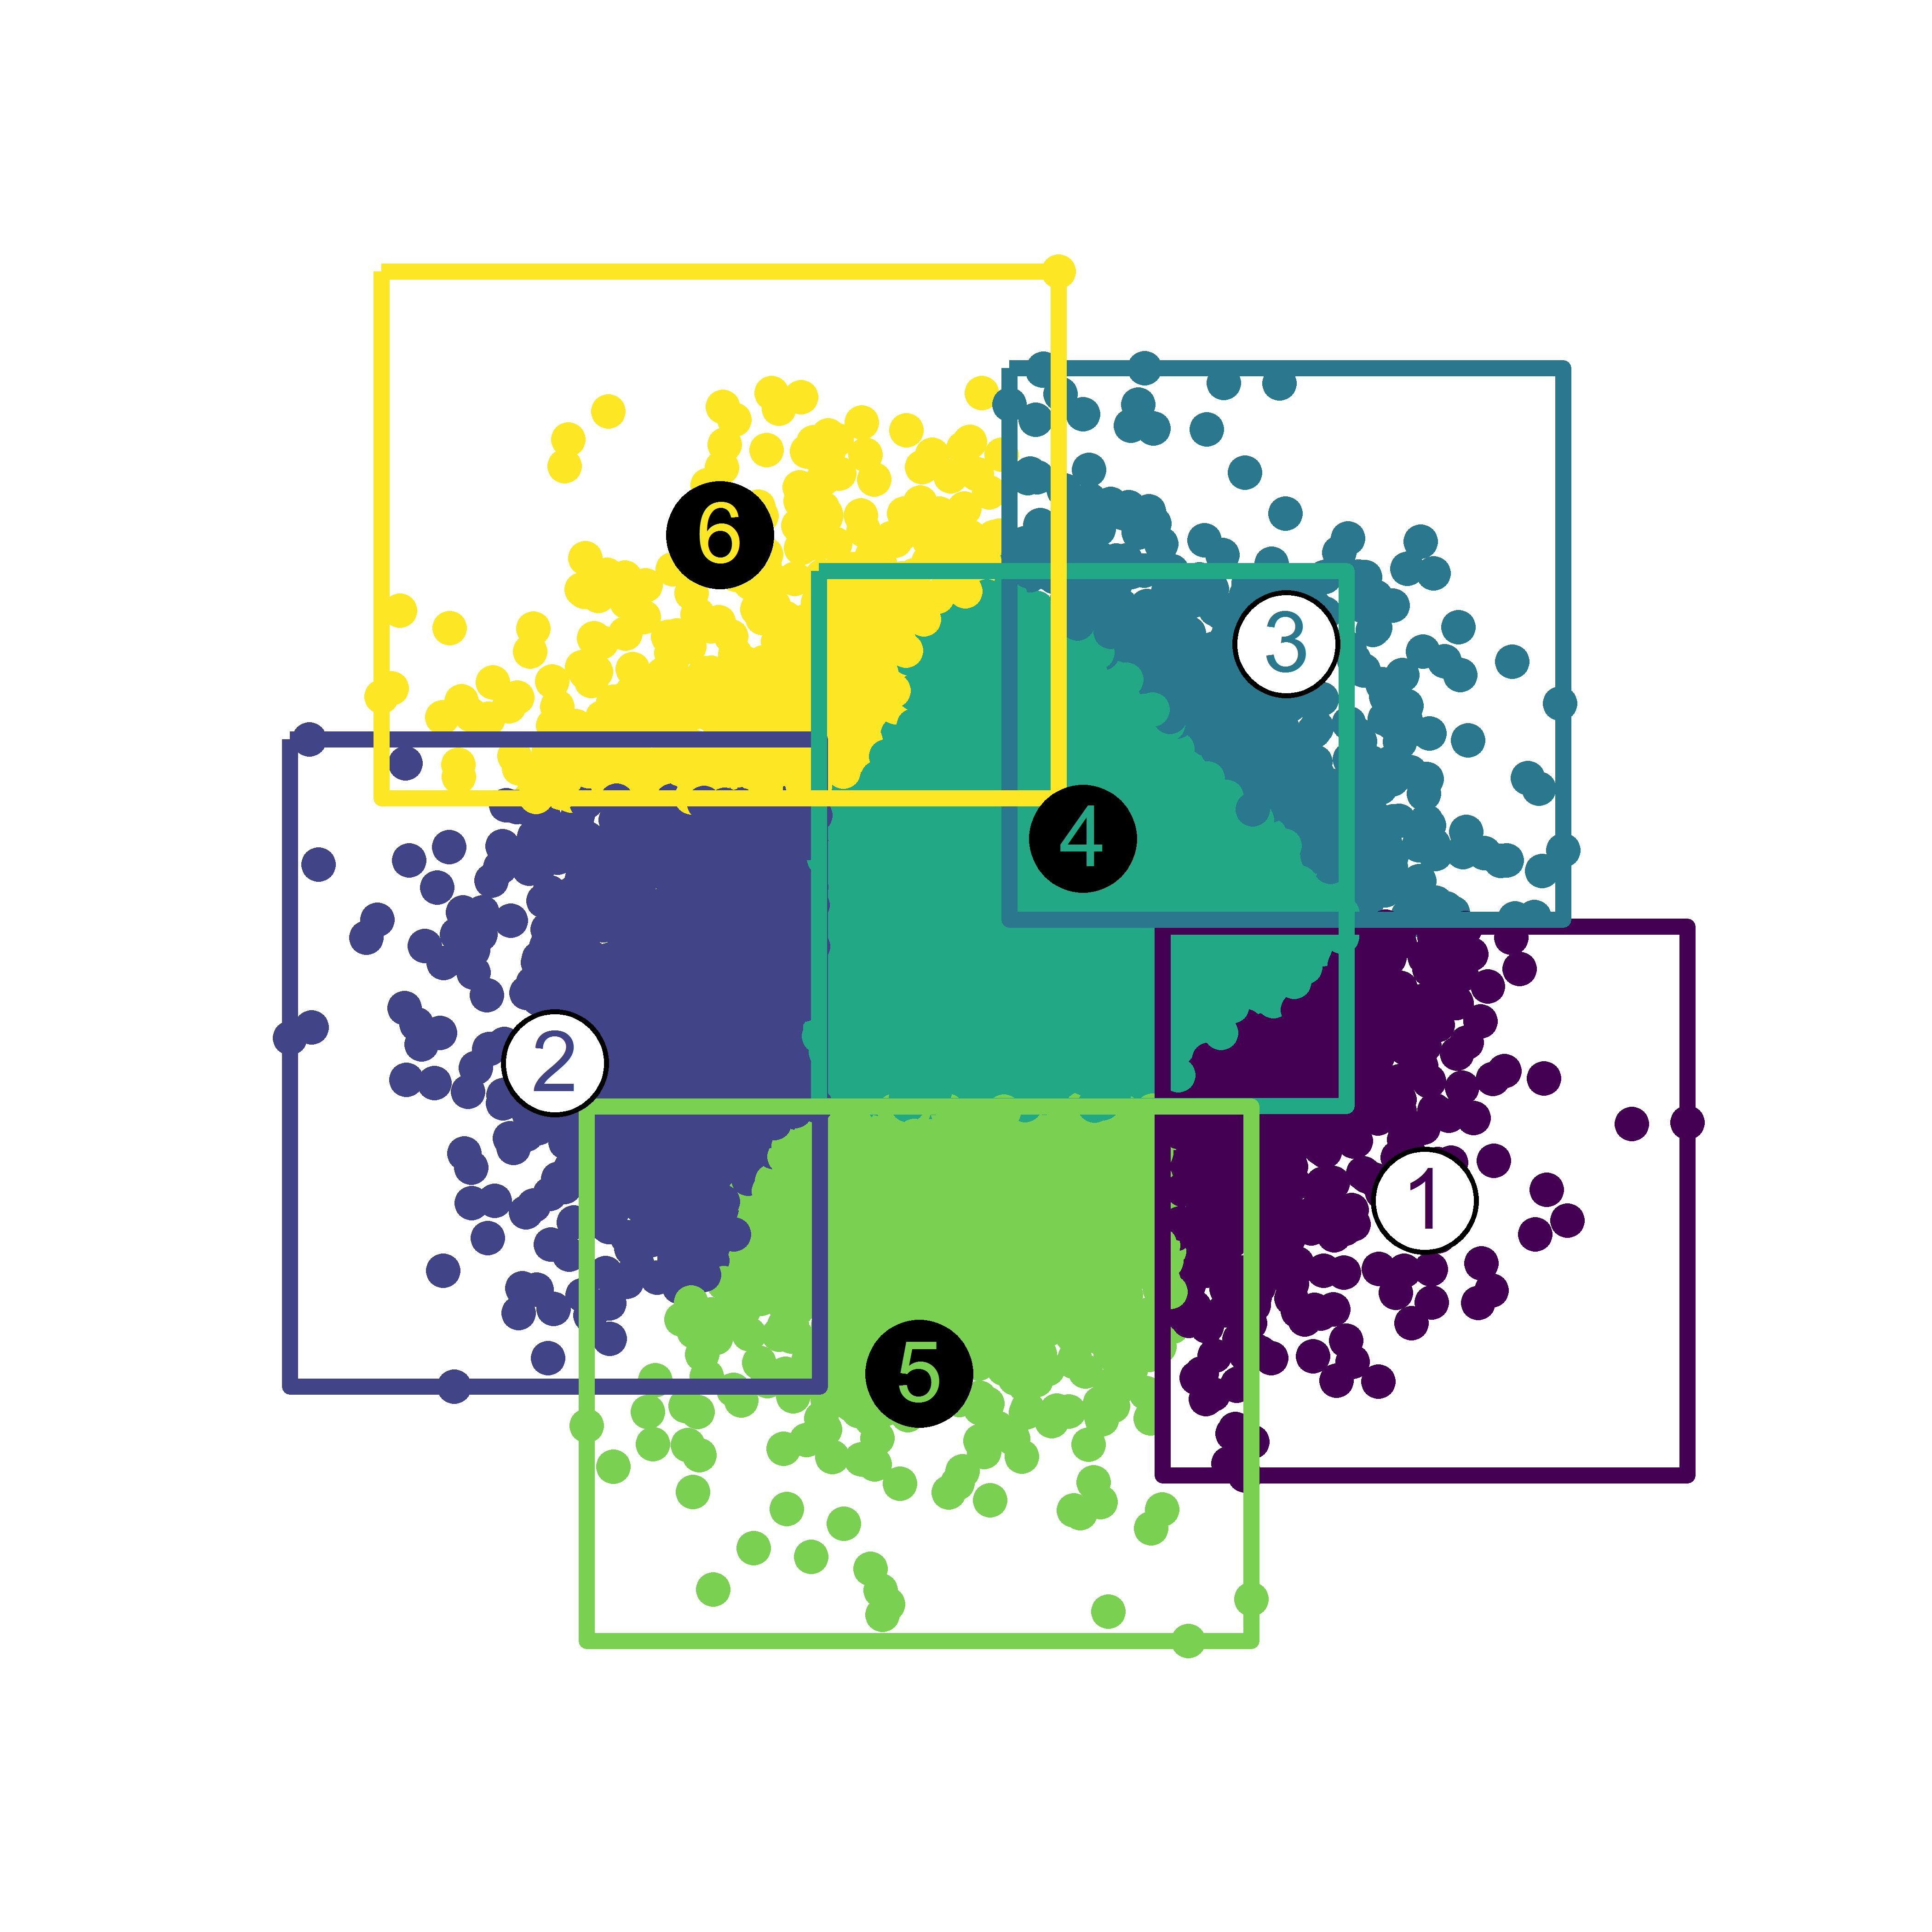
\includegraphics[width=0.4\linewidth]{figures/03_quantization/bsq_bbq_scatter/bbq_scatter.jpeg}
				}
				\caption[BSQ and BBQ examples]{The result of BSQ and BBQ on 2 dimensions of artificial data.}
				\label{fig:bsqbbqexample}
			\end{figure}
			
			Much like the approximation error, the difference between the $L_2$ and $L_\infty$ distance for two points can be arbitrarily large given enough dimensions.
			Since the goal was to use \ac{BBQ} as a fast approximation of \ac{BSQ}, especially in higher dimensions, this difference could pose a problem to the usefulness of the algorithm.
			Table~\ref{tab:bsbq} shows the results of running both \ac{BSQ} and \ac{BBQ} on the same datasets.
			The data points were generated the same way as for Fig.~\ref{fig:boxworstsets}, creating \textit{d} dimensional normal distributions with \textit{n} number of points.
			The algorithms were run multiple times for each parameter set, with the training points regenerated, and both algorithms starting from the same initial positions, with a target of $k = 10$ quanta.
			The results show well-contained approximation errors that are in-line with the measurements in Fig.~\ref{fig:boxrealsets}, and small differences in maximum quantization errors.
			\ac{BBQ} was considerably faster than \ac{BSQ} in most cases, especially for higher \textit{d} and \textit{n}.
			As expected, \ac{BBQ}'s runtime scales roughly linearly with both \textit{d} and \textit{n}, while the fitting of minimal bounding spheres in \ac{BSQ} makes the runtime scale superlinearly with both parameters.
			Based on this, \ac{BBQ} seems to be a good alternative to \ac{BBQ} in cases where runtime is critical, or where there is limited computational power available.
			
			\begin{table}[ht]
				\centering
				\begin{tabular}{|c|c|c|c|c|c|c|c|c|c|}
					\hline
					& & \multicolumn{2}{c|}{Runtime [seconds]} & \multicolumn{2}{c|}{Iterations} & \multicolumn{2}{c|}{Max. quant. err.} & \multicolumn{2}{c|}{Appr. err. [R]} \\
					d       & n         & BSQ       & BBQ     & BSQ     & BBQ       & BSQ       & BBQ       & Avg.      & Max. \\ 
					\hline
					$16$   	& $10^3$	& $0.07$   	& $0.08$  & $8.9$   & $9.4$  	& $4.978$  	& $6.142$  	& $0.4792$ 	& $0.6256$ \\
					$16$   	& $10^4$ 	& $0.23$   	& $0.16$  & $10.0$  & $11.2$ 	& $5.594$  	& $7.157$  	& $0.4056$ 	& $0.5504$ \\
					$16$   	& $10^5$ 	& $2.36$  	& $1.26$  & $11.0$  & $13.2$ 	& $6.031$  	& $7.902$  	& $0.3874$ 	& $0.5020$ \\
					$256$  	& $10^3$ 	& $0.84$    & $0.15$  & $10.5$  & $9.2$  	& $17.036$ 	& $19.005$ 	& $0.4342$ 	& $0.5798$ \\
					$256$  	& $10^4$ 	& $9.24$  	& $1.65$  & $12.9$  & $14.3$ 	& $17.629$  & $20.079$  & $0.4031$  & $0.4357$ \\
					$256$  	& $10^5$ 	& $131.58$ 	& $17.36$ & $12.4$  & $16.2$ 	& $18.111$	& $21.262$  & $0.4482$  & $0.4832$ \\
					$1024$ 	& $10^3$ 	& $9.97$ 	& $0.34$  & $8.6$   & $7.1$  	& $32.814$  & $35.402$  & $0.3889$ 	& $0.5479$ \\
					$1024$ 	& $10^4$ 	& $125.62$ 	& $5.76$  & $17.9$  & $13.6$    & $33.476$ 	& $36.551$  & $0.3515$ 	& $0.3744$ \\
					$1024$ 	& $10^5$	& $1252.80$	& $75.86$ & $16.5$  & $17.9$    & $34.033$  & $38.012$  & $0.3976$ 	& $0.4146$ \\
					\hline
				\end{tabular}
				\caption[BSQ and BBQ statistics]{BSQ and BBQ statistics.}
				\label{tab:bsbq}
			\end{table}
			
			In this work, for \kmeans{}, \ac{BSQ} and the \ac{BBQ} algorithms, we used our own implementations based on the \textit{R}\footnote{https://www.r-project.org/} programming language.
			For the \ac{1NN} classification in the expectation step, we used the \textit{nn2()} function implemented in the \textit{RANN}\footnote{https://cran.r-project.org/web/packages/RANN} package.
			Fischer's algorithm for fitting minimal bounding spheres in \ac{BSQ}'s maximization step was implemented in the excellent \textit{miniball}\footnote{https://github.com/hbf/miniball} library.
			
		\subsection{Similar Problems and Algorithms}
			\label{cha:quantization:sec:related}
			
			The problem addressed in this work is the $k$-center or minimax facility location problem, where to goal is to place $k$ centroids onto a group of points, in a way that achieves the lowest maximum distance to the points closest to them.	
			This problem is of course not limited to mobile networks, in fact it has been researched quite extensively since its first formulation for $2$ dimensions more than a century ago \cite{farthestfirst}.
			On one hand, there exist a few algorithms that solve the same problem, although not in the same way as our algorithm.
			On the other hand, there also exist algorithms that work very similarly to \ac{BSQ} and \ac{BBQ}, and solve similar, but not identical problems.
			This section assesses such algorithms and problems, in an attempt to clear possible confusion stemming from these similarities.
			
			Given $n$ observations, the \kmeans{} algorithm aims to find $k$ quantum centroids, for which the sum of quantization error for all observations is minimal.
			Two related problems to this are the \kmedoids{} and \kmedians{} formulations.
			Compared to \kmeans{}, \kmedoids{} chooses actual points from the data as quantum centroids.
			The most well known and widely used realization of \kmedoids{} is the \ac{PAM} algorithm \cite{kaufmanbook}.
			It can utilize arbitrary distance/dissimilarity metrics, originally designed to be used with $L_1$ metric.
						
			The \kmedians{} formulation is a variation of \kmeans{}, where the quantum centroids are calculated as the median of the dimensions instead of the mean.
			Medians are generally regarded as more statistically stable than means, which is why the \kmedians{} algorithm is often recommended as an alternative to \kmeans{}.
			Medians cause the algorithm to find quanta that are the most compact, since they minimize the sum of distances instead of the sum of squared distances, essentially using the $L_1$ distance instead of $L_2$.
			The \kmedoids{} and \kmedians{} formulations realize close to the same behavior as \kmeans{}, thus, they are not a solution for the $k$-center problem, and not a replacement for \ac{BSQ} or \ac{BBQ}.
			
			A simple and widely used algorithm to approximate the \textit{k}-center problem is the Farthest-First Traversal algorithm \cite{farthestfirst}.
			It works by always appending to a centroid set the farthest point from the centroid set, until $k$ quantum centroids are found.
			Although it is an approximating algorithm, it has polynomial runtime, and the approximation error can be quite large, at worst finding quanta with twice the minimal achievable radius.
			The algorithm is much greedier compared to \ac{BSQ}/\ac{BBQ}, creating quantizations that do not follow the shape or structure of the data well, however, it could be utilized as a preprocessing step to create the initial quantum set for our algorithms.
			
			A current approach to the \textit{k}-center problem is to use core-sets to extract a small set of points from the whole set, with which to approximate a good solution \cite{badoiu_approximate}.
			This approach is based on the same idea as \cite{kumar}.
			The authors present a $(1+\varepsilon)$-approximation algorithm, with a running time that has a linear dependency on the number of points, but exponential dependency on both $1/\epsilon$ (i.e. the accuracy of the method) and the number of centers.
			This algorithm lacks the advantages of the \ac{EM} framework, but has the added benefit that it has been extended to deal with noise points, to which the \textit{k}-center problem is very sensitive.
			
		\subsection{Experimental Results}
			
			Equal-volume quantization is designed on a compromise, where lower maximum error is traded for a higher overall quantization error.
			Except for edge-cases such as fully uniform distributions, \ac{BSQ} and \ac{BBQ} will usually produce a sub-optimal quantization when measured with one of the previously mentioned (Sec. \ref{cha:quantization:sec:high_dim_problem}) algorithms' optimization measures, and vice versa.
			An example of this can be seen in Fig.~\ref{fig:kmeansbeanscomp}, which shows results for both \kmeans{} and \ac{BSQ} run on the same dataset.
			\ac{BSQ} successfully created quanta with lower maximum quantization error, whereas \kmeans{} excelled in reaching its own global target, creating a quantization with lower overall error.
			The charts showing the respective optimization targets are framed for both algorithms.
			As the average quantization error is always lower for \kmeans{} than for \ac{BSQ}, this also entails that the sum of errors is also lower.
			
			\begin{figure}[ht]
				\centering
				\subfloat[\kmeans{}]{
					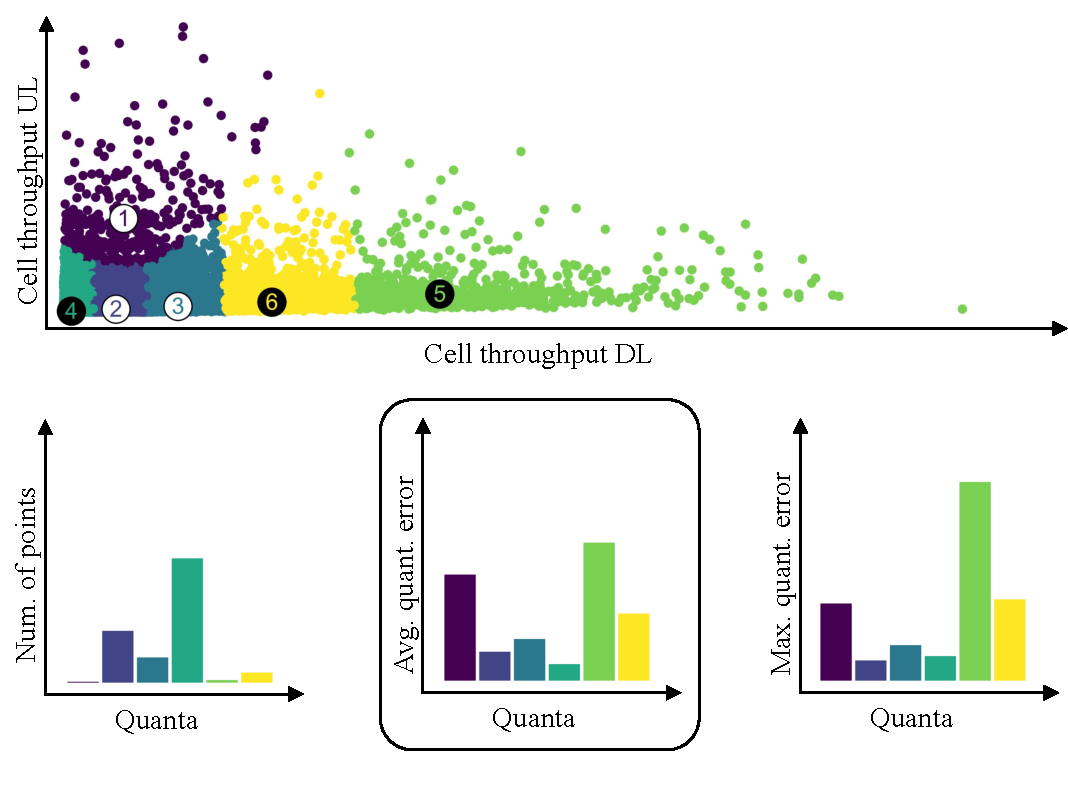
\includegraphics[width=0.48\linewidth]{figures/03_quantization/scatter_compare/scatter_compare_kmeans.pdf}
				}
				\subfloat[BSQ]{
					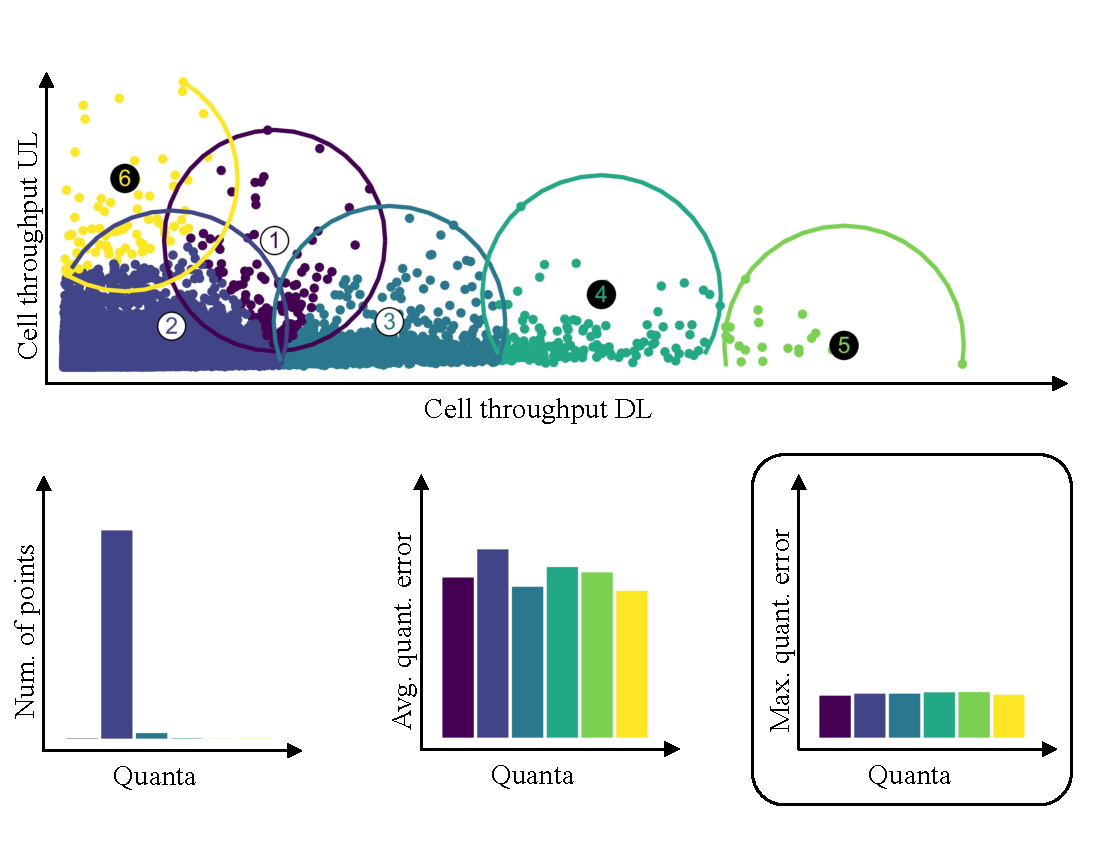
\includegraphics[width=0.48\linewidth]{figures/03_quantization/scatter_compare/scatter_compare_bsq.pdf}
				}
				\caption[\kmeans{} and BSQ comparison on $2$-dimensional data]{Comparison of \kmeans{} and BSQ on $2$ dimensions of PM data.}
				\label{fig:kmeansbeanscomp}
			\end{figure}
			
			We do not claim bounding volume quantization to be \textit{generally} better compared to these algorithms, only in specific use cases, such as visualization for data exploration.
			This use case was chosen to be shown here, because it is generic and can be illustrated well.
			In the following test, \ac{BSQ} and \kmeans{} was run on the same dataset consisting of $17$ \acp{KPI}, containing roughly $3$ months of measurements from more than $2000$ cells from a real mobile network
			The dataset was  made up of$4$ \acp{KPI} groups:
			\begin{itemize}
				\item \textbf{Demand}: Number of users, connection attempts/releases
				\item \textbf{Data}: Data volume, layer throughput, round-trip-times
				\item \textbf{Radio}: RSRP/Q, CQI, PRB utilization
				\item \textbf{Voice}: Voice data volume, number of QCI 1 users
			\end{itemize}
			\noindent 
			
			\begin{figure}[ht]
				\centering
				\subfloat[\kmeans{}]{
					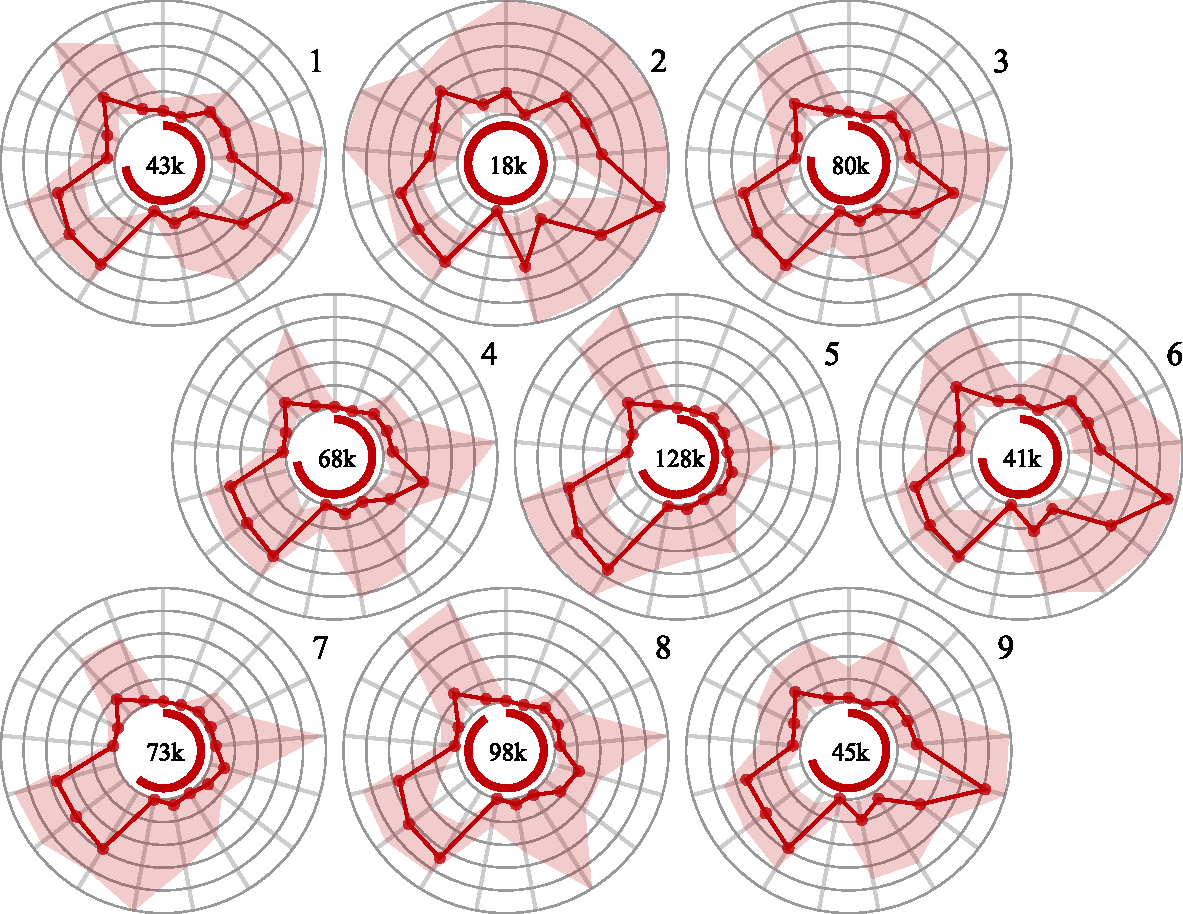
\includegraphics[width=0.48\linewidth]{figures/03_quantization/multidim_data/multidim_data_kmeans.pdf}
				}
				\subfloat[BSQ]{
					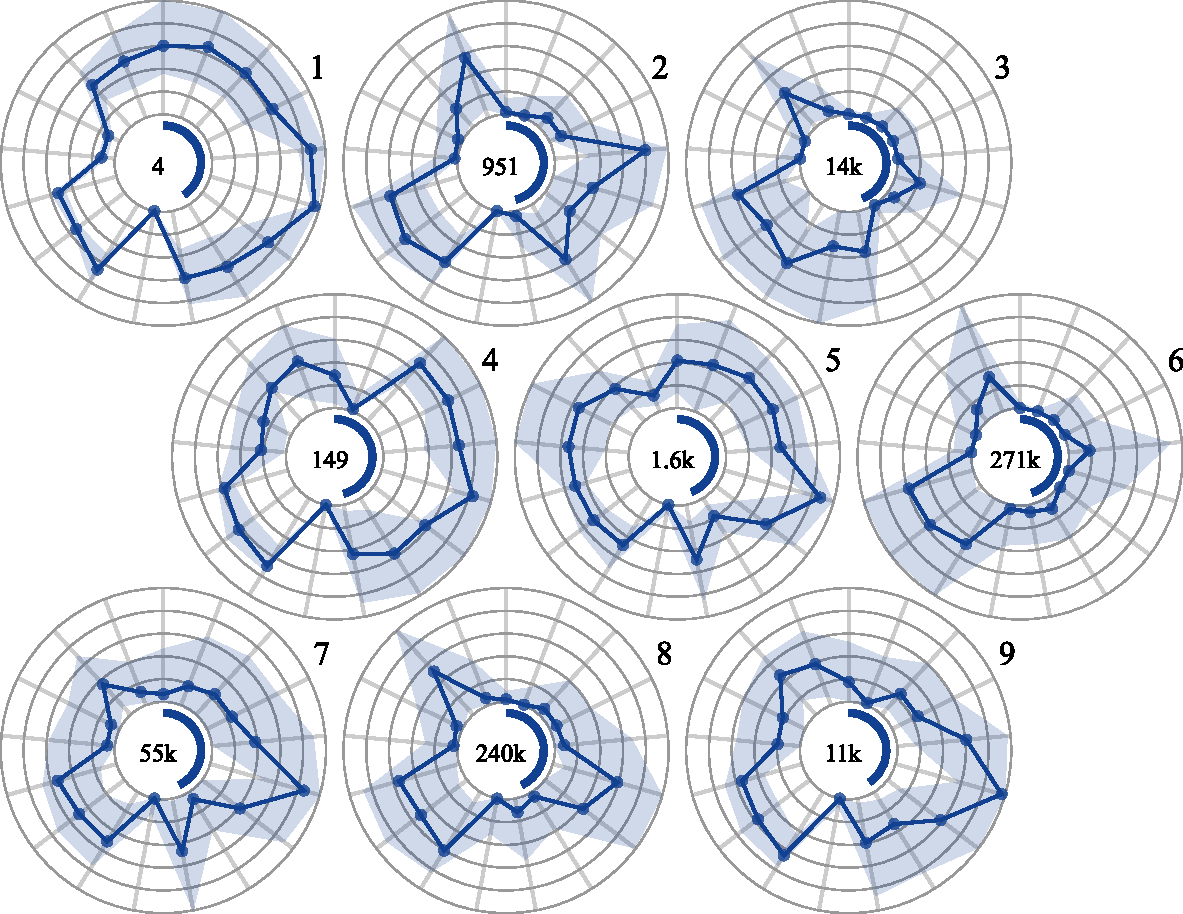
\includegraphics[width=0.48\linewidth]{figures/03_quantization/multidim_data/multidim_data_bsq.pdf}
				}
				\caption[\kmeans{} and BSQ comparison on high-dimensional data]{Comparison of \kmeans{} and BSQ on high-dimensional PM data}
				\label{fig:kmeansbeansmultidim}
			\end{figure}
			
			Figure~\ref{fig:kmeansbeansmultidim} shows the results of fitting $9$ quanta with both algorithms on the dataset, with the quantum centroids plotted as radar charts.
			The minimum and maximum values for each \ac{KPI} are plotted as a paler band, while the maximum quantization error is represented by the semi-circle on the inside.
			The numbers in the middle of the charts show the amount of measurements assigned to each quanta.
			As argued before, \kmeans{} by nature produces quanta that have largely varying assigned volumes, which is unintuitive for data exploration purposes.
			\ac{BSQ} creates much more evenly-sized (and indeed smaller in volume) quanta which lend better to human expectations.
			
			The \kmeans{} algorithm also produces very generic, ``uninteresting'' quanta, which do not properly explore the state space.
			In the example in Fig.~\ref{fig:kmeansbeansmultidim}, \kmeans{} hides a lot of variety by focusing on the very dense parts of the input space, which do not hold that much diversity.
			An example can be seen on quanta $4$, $5$, $7$ and $8$: the per \ac{KPI} quantum center values are very close in each quanta, for the human eye there is not much difference between them.
			
		\subsection{Conclusion and Critique}
		
			In the conclusion of the original paper for this work, it is noted that \ac{BSQ} lacks in one aspect compared to \kmeans{}; \ac{BSQ} is prone to disregard class boundaries (groups present in the dataset), even if they are well separable, on account of its distribution-free nature.
			\kmeans{}, on the other hand, finds separated clusters more reliably.
			It became clear that this aspect is very important in quantization algorithms, even if the goal is not necessarily the correct identification of groups in the data.
			Ultimately, this led us down on a path which culminated in clustering algorithm researching, as discussed later (Part~\ref{part:association}).
			
			\acp{SOM} are often used for visualization because of their inherent ability to map any higher dimensional space to 2D, stemming from the 2D structure of nodes that retains neighbor relations throughout the algorithms iterations.
			However, the distances between the nodes can vary arbitrarily, so these neighbor relations might actually mislead the user instead of helping in understanding.
			A possible future research direction could have been to implement similar neighbor recognition functionality as a post-processing step after quantization.
			An early prototype of this can be seen in Fig.~\ref{fig:map_bsq}, where quantum centroids connected by a black line are identified as neighbors.
			\ac{BSQ} would have improved upon \acp{SOM} by keeping the distances between nodes similar, thus being producing a intuitive mapping.
			Ultimately, our research moved in the direction of \ac{DL}, where encoding nets project the data into a low-dimensional space as a preprocessing step for quantization algorithms.
			At the time, our belief was that for visualization, the preprocessing can be effectively used to project the data directly into $2$D, alleviating the projection problem that \ac{SOM} attempts to solve.
			
			\begin{figure}[ht]
				\centering
				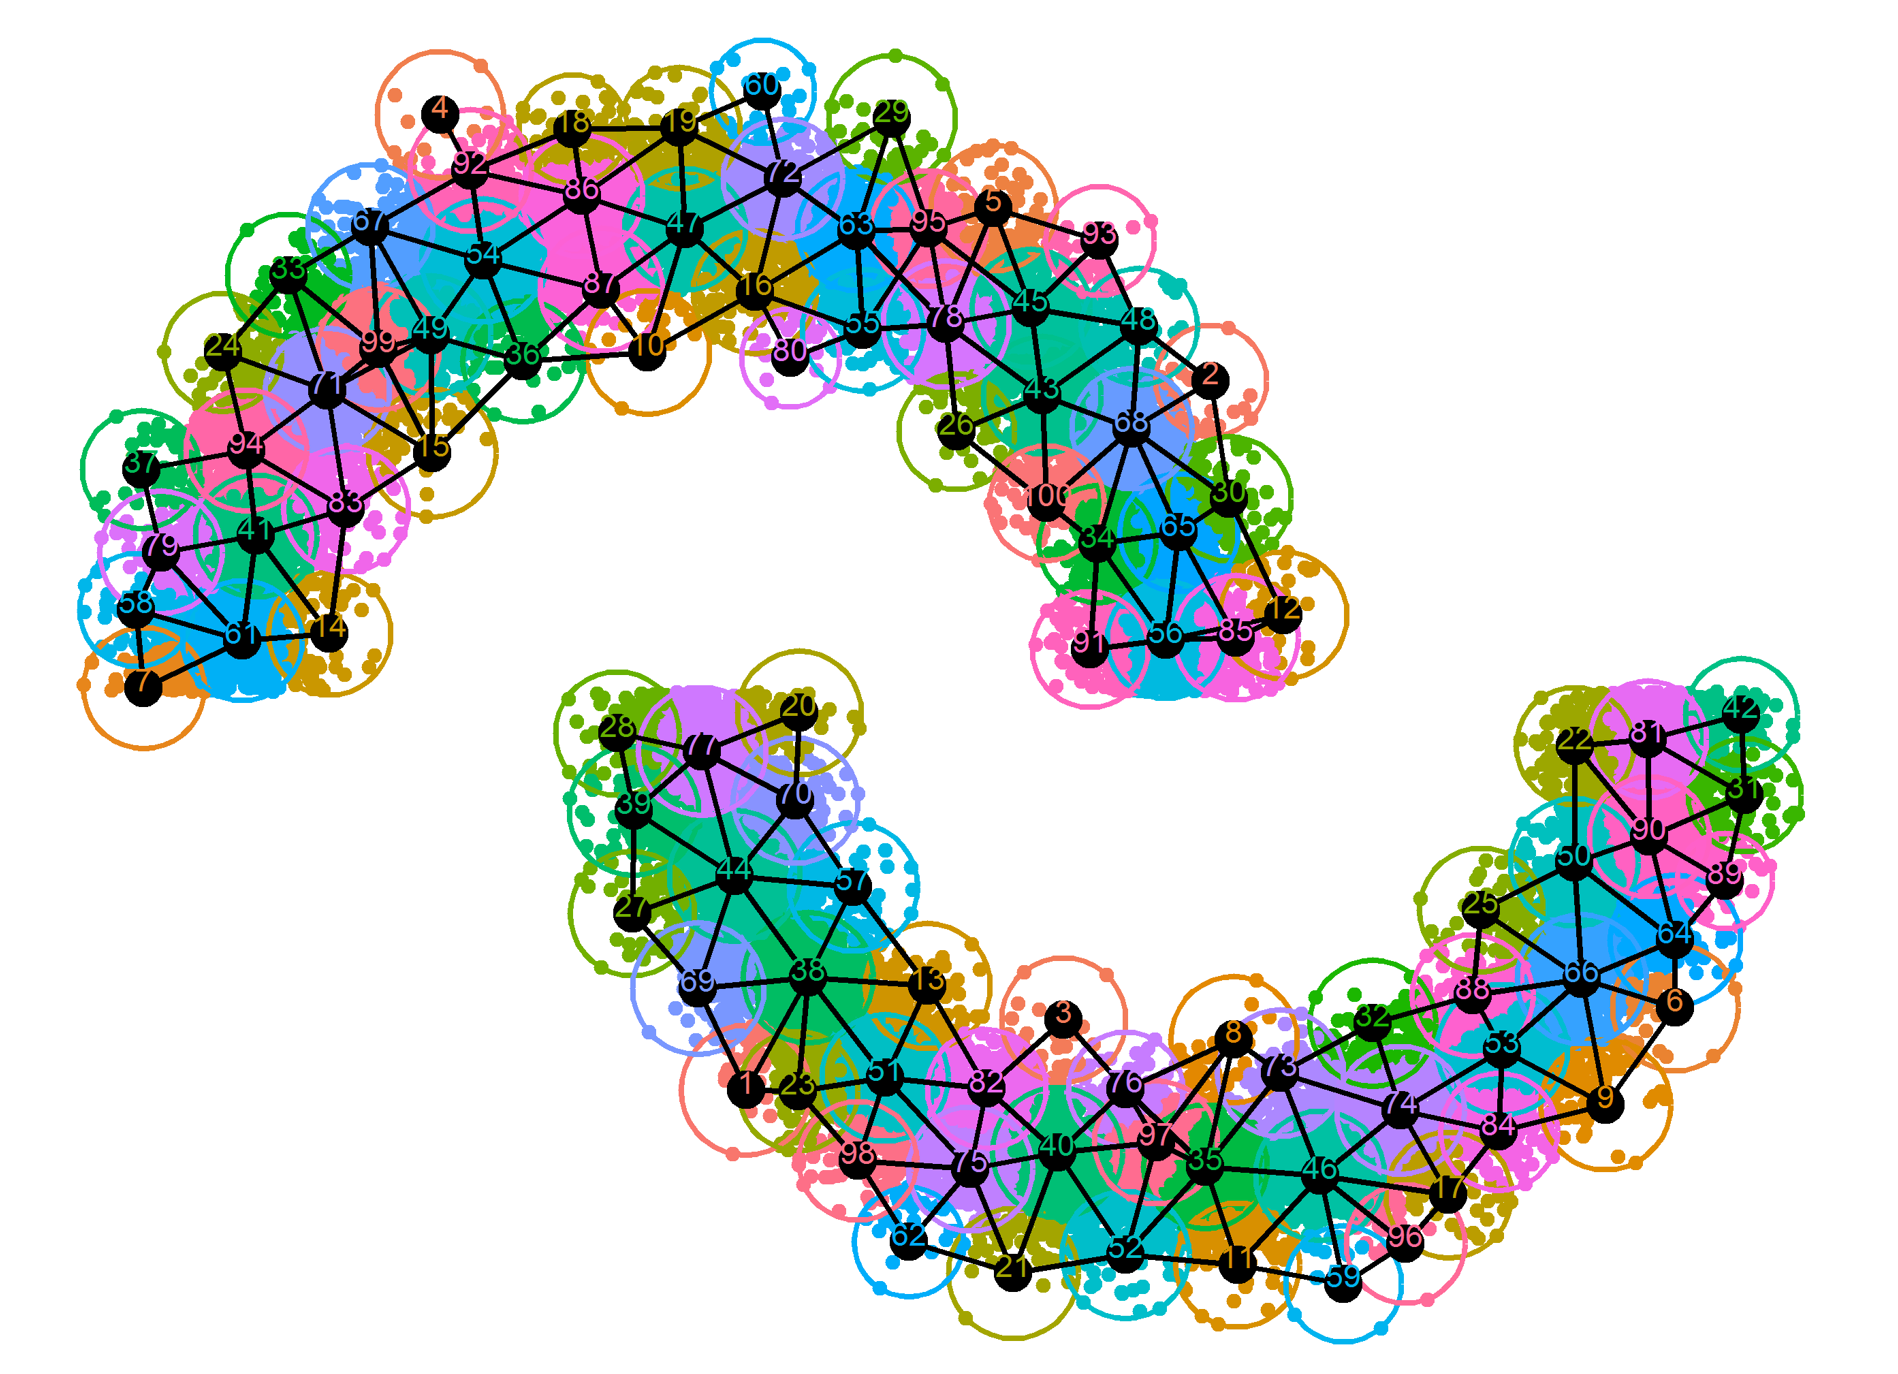
\includegraphics[width=0.6\linewidth]{figures/03_quantization/map_bsq/map_bsq.png}
				\caption[BSQ super-cluster prototype]{Early prototype of a BSQ quantization post-processed to form a neighbor-relation graph.}
				\label{fig:map_bsq}
			\end{figure}
			
			\ac{BSQ} and \ac{BBQ} can be categorized as more traditional, statistical \ac{ML} algorithms, far from the complex \ac{DL} algorithms that will be introduced later in this thesis.
			Nevertheless, these simple, lightweight algorithms are often used in combination with \ac{DL}, where \ac{DL} is used to simplify and project the data into an encoding space, which is then easily processed by these statistical algorithms, especially \kmeans{}.
			Unfortunately, there is a certain aspect of \ac{BSQ} which does not synergize well with such hybrid \ac{DL} and statistical \ac{ML} setups; stemming from its double optimization loops, \ac{BSQ} is quite computationally taxing to train.
			Often, these setups require the simple \ac{ML} algorithm to be run quite frequently, sometimes even multiple times for a single iteration of the \ac{DL} training (epoch).
			For \ac{BSQ} to be usable in such a setting, it has to be lightweight, with good scaling for both number of input points and number of quanta.			
			While we tried to address this issue in this work by proposing the simplified \ac{BBQ} alternative, we did not find it sufficiently accurate in later trials.
			However, we were able to achieve a significant speedup by implementing \ac{BSQ} with massive parallelization in mind, the topic of the next section.
			
	\section{Neural-Net-Based Quantization}
		\label{cha:quantization:sec:nn_quant}
			
		\subsection{Algorithms Designed for Massive Parallelization}
			
			Algorithms developed before the deep learning boom were almost explicitly implemented to be run on \acp{CPU}, considering only a handful of execution threads ($4$-$8$), and presuming that the operative memory, however quick, was still somewhat slow to access compared to compute operations.
			This motivated researchers to apply preprocessing techniques, such as speeding up searches in data structures (an example of which are $k$-dimensional-trees for nearest neighbor search \cite{ann}).
			However, these preprocessing stages often break parallelization.
			One approach is to duplicate the preprocessed structures for each thread of execution, which can lead to large memory utilization and a large overhead at the start of the algorithm.
			The other approach is to share the preprocessed structures between threads, which often breaks concurrency, as the threads have to wait on each other.
			At the time these issues were not in the spotlight, because hardware was generally not capable of significant parallelization.
			
			The introduction of dedicated massively parallel hardware accelerators -- \acp{GPU} -- and \acp{API} allowing the use of these accelerators for generic computation -- \ac{GPGPU} -- changed this paradigm.
			\acp{GPU} have thousands of computational cores and can effectively realize hundreds of parallel threads of execution, as well as having a relatively large amount of memory which is quick to access (much faster than operative memory).
			All of these features are there to facilitate massive parallelism: the calculation of thousands of simultaneous simple mathematical operations on data structures which are shared between execution threads, thus not needing a large amount of memory space.
			\acp{GPU} are designed for tensor ($n$-dimensional matrix) operations, such as calculating projections for rasterization.
			These operations mostly fall under linear algebraic or element-wise operations, such as addition or multiplication, min/max searches or simply indexing.
			If an algorithm is defined using only these simple operations, deep learning frameworks can automate the parallelization and data transfer in order to fully utilize a \ac{GPU}'s processing power.
			Often, running an algorithmically unoptimized algorithm in such a massively parallel environment can still result in a speedup compared to optimized, but only somewhat parallel execution on \acp{CPU}.
			
			Neural nets inherently use such simple algebraic operations, thus making them a perfect fit for \ac{GPU}-based hardware acceleration.
			However, other types of algorithms can also take advantage of this acceleration, if they can be broken down into these simple operations.
			This section describes such an implementation of \kmeans{} and \ac{BSQ} using \ac{GPU}-accelerated operations, organized into two main components, which act as layers in a neural net.
			
		\subsection{Implementation Overview}
			
			The biggest change in moving the \kmeans{} and \ac{BSQ} algorithms to a neural-net-based logic is the switch from the \ac{EM} optimization framework to stochastic gradient descent.
			For \ac{SGD} to work, the distance calculations need to produce a single loss value, that is to be backpropagated to update the quantum centroids.
			Selecting which of the distances between quantum centroids and training points contribute to the loss value differentiates between \kmeans{} and \ac{BSQ}.
			Both the distance calculation and the distance selection can be realized as neural net layers.
			Additionally, the stochastic nature of batching breaks \ac{BSQ}, so a cross-batch accumulation is required.
			This accumulation, however, can also benefit \kmeans{}.
			An overview of the whole process can be seen in Fig.~\ref{fig:quant_overview}, whose individual steps are discussed in the following sections.
			
			\begin{figure}[ht]
				\centering
				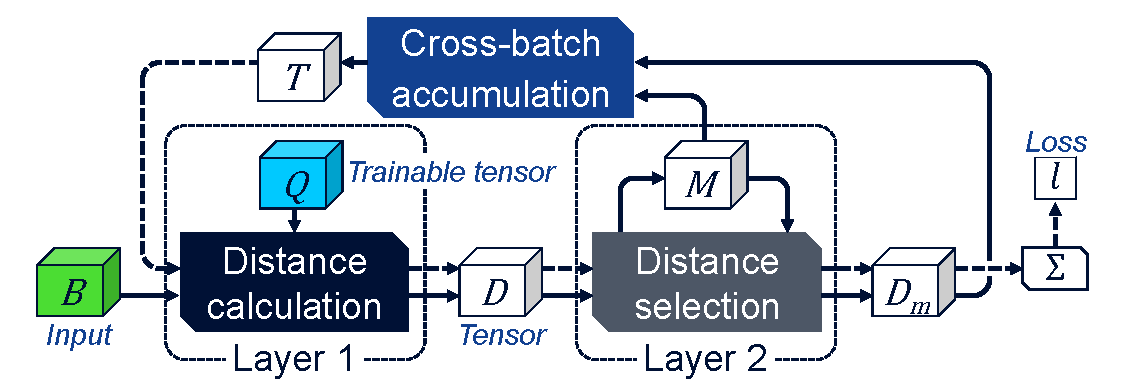
\includegraphics[width=0.75\linewidth]{figures/03_quantization/quant_overview/quant_overview.pdf}
				\caption[Neural-net-based \kmeans{} and BSQ processing steps]{Overview of the processing steps for \kmeans{} and \ac{BSQ} implemented as a neural-net.}
				\label{fig:quant_overview}
			\end{figure}
			
		\subsection{Distance Calculation Layer}
			
			The core of \kmeans{}-like quantization is a calculation of distance, measured between training points and quantum centroids.
			For this work, we consider $p$-norms only, as these cover the most commonly used distances, such as the $L_2$ (Euclidean distance, or $2$-norm), upon which both \kmeans{} and \ac{BSQ} is built.
			PyTorch and TensorFlow includes ready implementations of calculating $p$-norms of vectors organized into tensors (multi-dimensional matrices), but complete functions to calculate set-to-set distances between two set of points were missing from both libraries at the time.
			To overcome this, \textit{broadcasting}, a technique that is available in both libraries can be used, which enables the calculation of all set-to-set distances without the need to manually duplicate data in memory.
			
			Let $B$ (batch) be a tensor of shape $(n\: rows, d\: columns)$ containing training points, where $n$ is the size of the current batch, and $d$ is the number of dimensions.
			Let $Q$ be a tensor of shape $(k, d)$ containing $k$ quantum centroids.
			In this case, $B$ can be recast to shape $(n, d, 1)$ resulting in tensor $B'$, and $Q{^T}$ (the transpose of $Q$) can be recast to shape $(1, d, k)$ resulting in tensor $Q{^T}'$ without any memory copies created.
			The tensor dimensions of size $1$ can then be reused (broadcasted) without copy in the element-wise subtraction $B' - Q{^T}' = D'$.
			The resulting tensor $D'$ with shape $(n, d, k)$ contains all pairwise difference vectors between $B$ and $Q$.
			Finally, the pairwise distances between $B$ and $Q$ can be calculated by computing the $p$-norm of $D'$ in the direction of the middle tensor dimension of size $(d)$, reducing $D'$ into $D$ with shape $(n, k)$.
			The operation can be seen in Fig.~\ref{fig:distance_calc}.
			
			\begin{figure}[ht]
				\centering
				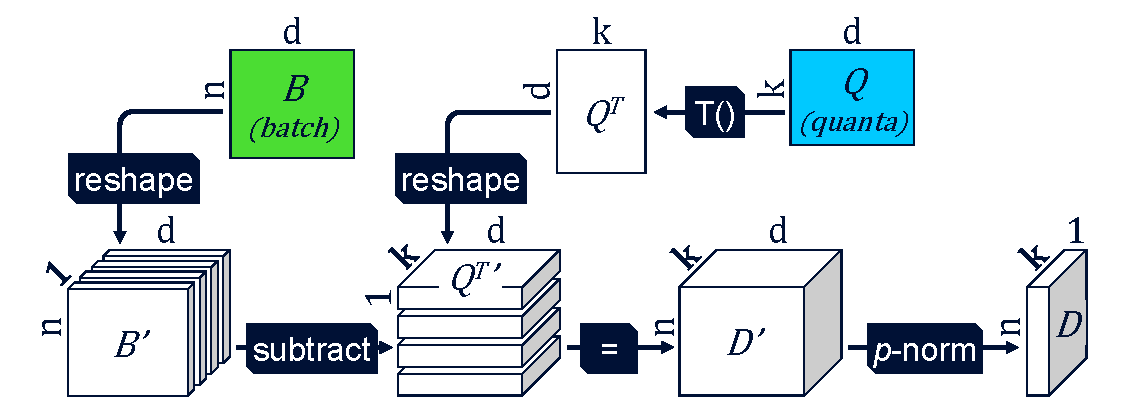
\includegraphics[width=0.75\linewidth]{figures/03_quantization/distance_calc/distance_calc.pdf}
				\caption[Neural-net-based \kmeans{} and BSQ distance calculation]{Distance calculation steps.}
				\label{fig:distance_calc}
			\end{figure}
			
		\subsection{Distance Selection Layer}
			
			For both algorithms, only the distances to the closest quantum centroid should contribute to the final loss value.
			This translates into the need of selecting the smallest distance for each training point, which is a row-wise minimum search in tensor $D$.
			However, cross-batch accumulation needs to retain information about which distance belongs to which quantum, so instead of selecting the smallest values, it is better to mask all other unimportant distance values by multiplying them with $0$.
			To do this, the masking tensor $M$ of shape $(n, k)$ is created, which contains $1$-s at places where $D$ contains row-wise minima, and $0$-s everywhere else.
			Element-wise multiplying $D * M = D_m$ results in the masked distance tensor $D_m$ with shape $(n, k)$.
			The operation can be seen in Fig.~\ref{fig:distance_select}.
			
			\begin{figure}[ht]
				\centering
				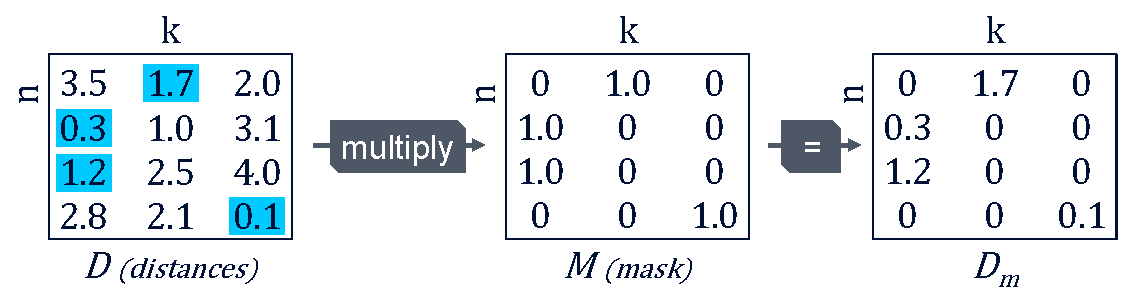
\includegraphics[width=0.75\linewidth]{figures/03_quantization/distance_select/distance_select.pdf}
				\caption[Neural-net-based \kmeans{} and BSQ distance selection]{Distance selection through masking.}
				\label{fig:distance_select}
			\end{figure}
			
		\subsection{Cross-Batch Accumulation}
			
			To be clear, the step of cross-batch accumulation is not necessary for \kmeans{}.
			Because a large-enough random sample from a set of points retains the distribution of the original set with a high confidence, the stochastic samples contained within the batches likely have the same mean as the whole set of training points (weak law of large numbers \cite{lawOfLarge}).
			Because of this, for \kmeans{} it is enough to calculate the mean of the $D_m$ tensor and backpropagate this value as the final loss in every iteration.			
			However, this is not true for \ac{BSQ}.
			Finding the farthest point in each batch for each quanta, and trying to minimize those distances will not result in a similar behavior as finding the farthest points in the whole training set.
			To overcome this, the optimization targets are accumulated across batches, and the quantum centroids are only updated after a certain number of batches were processed.
			The number of batches to be processed before each update is the user-set parameter $r$.
			In case of $r = n_{batches}$, there is no accumulation (updates happen at every batch), whereas for $r = 1$, updates only happen after all batches were accumulated (once every epoch).
			Early in the quantization training, the rough estimate gained by true \ac{SGD} (large $r$ value) is good enough for both algorithms, as the quantum fits are anyway not optimized yet.
			By the end of the training, where precise fitting is needed, $r=1$, so that updates happen on fully accumulated results, basically turning the optimization into (non-stochastic, regular) Gradient Descent.
			
			To realize accumulation, when not updating, a target tensor $T$ (target) of shape $(k, d)$, and a corresponding weight tensor $W$ of shape $(k)$ is maintained.
			During the update, tensor $T$ is forward propagated as input through the layers, and the resulting masked distance tensor $D_m$ is summed to create a final loss value $l$.
			This $l$ is then backpropagated through the distance selection and masking layers to update the quantum centroids.
			
			For \kmeans{}, $T$ holds the running average of assigned training points for each quanta since the last update, while $W$ holds the number of training points that contributed to the running average.
			When forward propagating, in order to find which training points are assigned to which quanta, the mask $M$ from the distance selection layer can be used.
			For each column (quanta) in $M$, the position where a rows contains the value $1$, the value from the corresponding position in $B$ is used to calculate a batch and quantum-wide mean $T'$ $(k, d)$.
			The number of points that make up each mean can be computed by summing each column in $M$, and is stored in a temporary tensor $W'$ $(k)$.
			Each row in tensor $T$ is then updated according to:
			\begin{equation}
				T[i] = \frac{W[i] * T[i] + W'[i] * T'[i]}{W[i] + W'[i]},
			\end{equation}			
			\noindent where $[i]$ refers to the corresponding subset along the first tensor dimension, i.e. row or single value.
			$W$ is updated according to $W = W + W'$. 
			
			For \ac{BSQ}, $T$ holds the so far found farthest training point for each quanta, where as $W$ holds the distance of said point to the corresponding quantum, while $T'$ and $W'$ are equivalent tensors for the current batch.
			Both can be generated by selecting the row from $B$ where (for each column) the value in $D_m$ was the largest; the rows from $B$ make up $T'$, while the largest values from $D_m$ make up $W'$.
			Now, the row $T[i]$ is overwritten with $T'[i]$, if $W'[i] > W[i]$.
			Similarly, $W[i]$ is also overwritten with $W'[i]$ in this case.
			The process of accumulation for both \kmeans{} and \ac{BSQ} can be seen in Fig.~\ref{fig:accumulate}.
			The values of tensor $W$ are set to $0$ after each update for both algorithms, to restart the accumulation of targets in $T$.
			
			\begin{figure}[ht]
				\centering
				\subfloat[\kmeans{}]{
					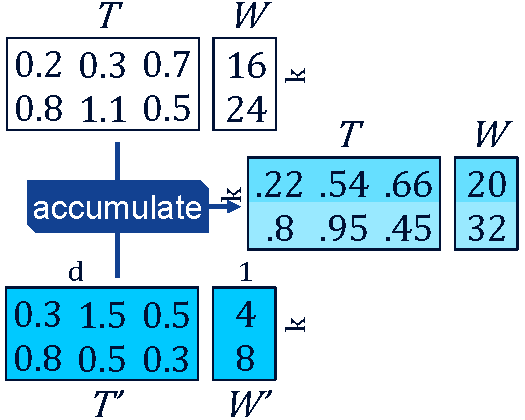
\includegraphics[width=0.35\linewidth]{figures/03_quantization/accumulate/accumulate_kmeans.pdf}
				}
				\hspace{0.1\textwidth}
				\subfloat[\ac{BSQ}]{
					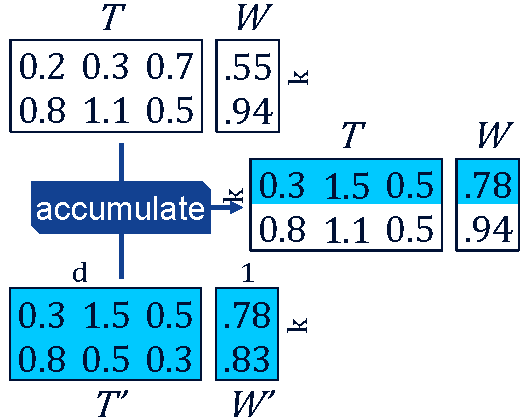
\includegraphics[width=0.35\linewidth]{figures/03_quantization/accumulate/accumulate_bsq.pdf}
				}
				\caption[Neural-net-based \kmeans{} and BSQ accumulation]{\kmeans{} and BSQ accumulation examples.}
				\label{fig:accumulate}
			\end{figure}
			
			Both the accumulation and the use of \ac{SGD} are critical components for the correct functioning of \ac{BSQ}.
			Accumulation makes it possible to find the true training-set-wide farthest points, while \ac{SGD} replaces the fitting of minimal bounding spheres present in the original \ac{BSQ}.
			As an illustration of how this works; when quantum centroids end up in the middle between two farthest points, \ac{SGD} moves the quantum centroid towards one of the farthest points in one iteration, and towards the other in the next, approximating the move towards the center of the minimal bounding sphere.
			Usually, by the end of the training, the learning rate is low, so the noise caused by this jitter is barely noticeable in the quantization.
			
		\subsection{Related Work and Evaluation}
			
			Large amount of research has been done with the aim of speeding up the original \kmeans{} algorithm.
			Among many ideas, the two most frequently utilized are the use of indexing schemes (such as $kd$-trees) to speed up search for the closest quanta \cite{kmeansKD}, and the use of the triangle inequality to avoid the calculation of distances whenever possible \cite{kmeansFaster, kmeansTriangle}.
			Although algorithmically faster, these ideas are complicated to realize in the massively parallel processing environment of a \ac{GPU}.
			A \ac{GPU} can potentially run parallel thread executions numbering in the ten thousands, for which the duplication of indexing structures (such as $kd$-trees) would be infeasible.
			The use of triangle inequality is not as simple to dismiss, and there have been successful implementations of this scheme that utilize a \ac{GPU} \cite{kmeansCuda}.
			However, the logic is very complex, and the speedup is heavily dependent on data ordering/structure.
			
			\ac{BSQ} is not a well-known algorithm, and as such, has not seen research regarding speedup yet.
			However, the core of the originally proposed \ac{BSQ}, the fitting of the minimal bounding sphere is a well-researched subject.
			Fischer's algorithm \cite{fischer} is the so far found quickest method, but due to many aspects, it is hard to implement it to run on a \ac{GPU}.
			
			Our \kmeans{} and \ac{BSQ} implementation was written in the Python language, utilizing the PyTorch library for \ac{GPU} acceleration.
			For reference, we chose a readily available \kmeans{} implementation that fits into this software environment from the SciPy\footnote{https://www.scipy.org/} library (\textit{scipy.cluster.vq.kmeans2}), which utilizes multi-threaded \ac{CPU} execution, but no \ac{GPU} acceleration.
			The evaluation was run on a system with an AMD Ryzen Threadripper 1920X 12-core \ac{CPU} with $64$ GB of memory, and an Nvidia GeForce 1080 Ti \ac{GPU} with $12$ GB of memory.
			
			Overall, training the \kmeans{} and \ac{BSQ} algorithms are not computationally heavy tasks (compared to for example training a state-of-the-art \ac{DNN}), so moving batches of data to and from the \ac{GPU} can create a significant overhead on smaller datasets.
			Conversely, large datasets usually do not fit into the limited memory of a \ac{GPU}, and the user is forced to keep the dataset in \ac{CPU} memory and process it batch-by-batch on the \ac{GPU}.
			In this evaluation, both batched and non-batched versions of the algorithms were measured, with the batched versions denoted as \ac{BSQ}$_b$ and \kmeans{}$_b$.
			The results can be seen on Tab.~\ref{tab:times}, where $k$ denotes the number of quanta fitted, and $n$ the number of training points.
			The training points were randomly generated from a $d$-dimensional normal distribution with $0$ mean and $1$ standard deviation.
			Each algorithm was run for a $100$ epochs.
			
			\begin{table}[t]
				\centering
				\setlength\tabcolsep{4pt}
				\begin{tabular}{|l|l|l|r r r r r|l}
					\cline{1-8}
					k							& n							&d					& \ac{BSQ}$_b$		& \kmeans{}$_b$ 	& \ac{BSQ}		& \kmeans{}		& SciPy				&		\\
					\cline{1-8}
					\multirow{9}{*}{$32$}		& \multirow{3}{*}{$10^3$}	& $10$				& $16.29$			& $16.12$			& $0.14$		& $0.15$		& $0.02$			&		\\
					\cline{3-3}
					& 							& $10^2$			& $16.53$			& $16.58$			& $0.11$		& $0.11$		& $0.05$			&		\\
					\cline{3-3}
					&							& $10^3$			& $16.93$			& $17.18$			& $0.41$		& $0.46$		& $0.49$			&		\\
					\cline{2-8}
					& \multirow{3}{*}{$10^4$}	& $10$				& $19.76$			& $19.93$			& $0.25$		& $0.16$		& $0.15$			&		\\
					\cline{3-3}	
					&							& $10^2$			& $20.11$			& $20.34$			& $0.48$		& $0.45$		& $0.56$			&		\\
					\cline{3-3}
					&							& $10^3$			& $22.79$			& $23.45$			&\hlone{$3.06$}	&\hlone{$3.81$}	&\hlone{$5.04$}		&\hlone{} 						\\
					\cline{2-8}
					& \multirow{3}{*}{$10^5$}	& $10$				& $43.85$			& $46.34$			&\hlone{$1.33$}	&\hlone{$0.64$}	&\hlone{$1.42$}		&\hlone{}						\\
					\cline{3-3}
					& 							& $10^2$			& $45.87$			& $48.79$			&\hlone{$3.74$}	&\hlone{$3.77$}	&\hlone{$5.77$}		&\hlone{\multirow{-3}{*}{$(1)$}}	\\
					\cline{3-3}
					& 							&$10^3$				&\hlthree{$69.97$}	&\hlthree{$75.22$}	& $-$			& $-$			&\hlthree{$49.54$}	&\hlthree{$(3)$}	\\
					\cline{1-8}
					\multirow{9}{*}{$512$}		& \multirow{3}{*}{$10^3$}	& $10$				& $16.96$			& $17.35$			& $0.22$		& $0.19$		& $0.18$			&		\\
					\cline{3-3}
					& 							& $10^2$			& $17.29$			& $17.39$			& $0.63$		& $0.74$		& $0.44$			&		\\
					\cline{3-3}
					& 							& $10^3$			& $21.67$			& $22.88$			&\hltwo{$5.18$}	&\hltwo{$6.44$}	&\hltwo{$3.29$}		&\hltwo{$(2)$}	\\
					\cline{2-8}
					& \multirow{3}{*}{$10^4$}	& $10$				& $18.92$			& $19.60$			& $1.01$		& $1.04$		& $2.02$			&		\\
					\cline{3-3}	
					& 							& $10^2$			&\hlfour{$24.26$}	&\hlfour{$25.08$}	& $-$			& $-$			&\hlfour{$4.42$}	&\hlfour{$(4)$}		\\
					\cline{3-3}
					& 							& $10^3$			&\hlthree{$70.19$}	&\hlthree{$82.23$}	& $-$			& $-$			&\hlthree{$29.26$}	&\hlthree{}		\\
					\cline{2-8}
					& \multirow{3}{*}{$10^5$}	& $10$				&\hlthree{$42.39$}	&\hlthree{$44.93$}	& $-$			& $-$			&\hlthree{$16.87$}	&\hlthree{}		\\
					\cline{3-3}
					& 							& $10^2$			&\hlthree{$83.01$}	&\hlthree{$99.08$}	& $-$			& $-$			&\hlthree{$40.05$}	&\hlthree{}		\\
					\cline{3-3}
					& 							& $10^3$			&\hlthree{$546.09$}	&\hlthree{$669.21$}	& $-$			& $-$			&\hlthree{$296.92$}	&\hlthree{\multirow{-4}{*}{$(3)$}}	\\
					\cline{1-8}
				\end{tabular}
				\caption[Neural-net-based \kmeans{} and BSQ statistics]{\kmeans{} and BSQ runtime statistics in seconds.}
				\label{tab:times}
			\end{table}
			
			Generally, the non-batched versions of \kmeans{} and \ac{BSQ} are quite competitive with the SciPy implementation, even winning in cases of low $k$ but high $n$ or $d$ values (highlighted as $1$).
			The SciPy implementation probably incorporates some form of speedup scheme (such as kd-trees, but there is no reference in the documentation), as its runtime does not scale linearly with $k$, and so it wins out for large values of $k$ ($2$).
			Dashes denote data sizes where the data and the net together no longer fit into the \ac{GPU} memory, and as such, non-batched versions of our algorithms were no longer feasible to run.
			
			Batched versions use a batch size of $512$.
			With this batch size, small datasets incurred such a heavy overhead that \ac{BSQ}$_b$ and \kmeans{}$_b$ could run several magnitudes slower than the SciPy or their non-batched counterparts.
			However, at the point where using the non-batched versions becomes infeasible, the batched versions are only $2x-3x$ slower than the SciPy implementation ($3$), except in the single worst case of ($4$).
			
		\subsection{Conclusion}
		
			This section proposed a neural-net-like implementation of the \kmeans{} and our \ac{BSQ} algorithms.
			While not achieving particularly groundbreaking speedup for \kmeans{}, the implementation did show some improvement with realistic parameters, where these algorithms are probably used.
			However, the main goal of this research, the runtime of \ac{BSQ} is greatly improved: while it is a little hard to compare, as the original implementations were measured for different number of iterations (Tab.~\ref{tab:bsbq}), the neural-net-based implementations (Tab.~\ref{tab:times}) show a huge improvement.
			Furthermore, undertaking the research detailed in this section gave me valuable insight into the benefits and downsides of using massively parallel algorithms, which I think is applicable to all \ac{DL} algorithms in similar settings.
			Thus, in the next section, I would like to conclude some general remarks about important aspects of the use of massively parallel algorithms. 
		
	\section{On Massively Parallel Algorithms in Mobile Networks}
		\label{cha:quantization:sec:on_parallelization}	

		The utility of every algorithm is tied to ease of use, a large part of which is simply runtime.
		Algorithms which take a long time to train are slower to iterate upon, or do not get the necessary training time to fully converge, and thus, never reach their full potential.
		This is especially true for simple \ac{ML} algorithms -- such as \kmeans{} and \ac{BSQ} -- which are often utilized as part of a larger algorithm, such as a \ac{DNN}.
		The neural-net-based implementations of \kmeans{} and \ac{BSQ} highlighted the importance of designing for scalability and integration into larger \ac{DL} environments.
		
		In the batched case, the runtime of \ac{BSQ} contains a considerable amount of overhead from data transfers, as each batch of data has to be moved from the \ac{CPU} memory to the \ac{GPU} memory.
		Because the batch size limits the amount of calculations that are required at any given time (and because the calculations themselves are pretty simple), the overhead from data transfer can make up the majority of the runtime in some cases.
		However, as we will see later, we often used quantization algorithms as part of a \ac{DNN} training, where for every \ac{SGD} iteration of the \ac{DNN}, the quantization algorithm is also trained (usually until it converges).
		Such a scenario is depicted in Fig.~\ref{fig:dnn_quant}, where \kmeans{} is trained on the encoded, latent representation in an autoencoder, together (in parallel) with the whole autoencoder.
		In this case, as the data already has to be transferred to the \ac{GPU} for the encoding process, using a \ac{CPU}-based implementation actually means needing an additional data transfer between \ac{GPU} and \ac{CPU}, whereas if a \ac{GPU}-based implementation is used, this transfer can be spared.
		In these scenarios, even if the \ac{GPU}-based implementation is not as optimized as the \ac{CPU}-based, the reduction in overhead could mean quite the speedup between the implementations.
		
		\begin{figure}[ht]
			\centering
			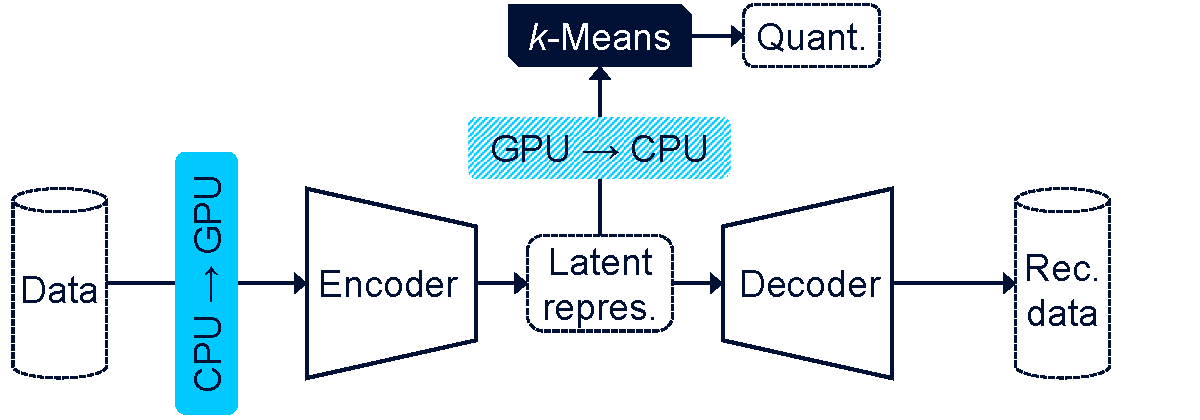
\includegraphics[width=0.8\linewidth]{figures/03_quantization/dnn_quant/dnn_quant.pdf}
			\caption[Data transfers in DNN training]{Data transfers in parallel training of a DNN and \kmeans{}.}
			\label{fig:dnn_quant}
		\end{figure}
		
		In the above scenario, there are additional factors which could further worsen the ratio between useful computation time and overhead.
		Both \kmeans{} and \ac{BSQ} can be initialized with previously found quantum centroids, and the training can be continued where it left off in the previous epoch.
		As the autoencoders are trained with \ac{SGD}, early in the training the encoded observation likely change a lot between each epoch, thus the quantization algorithms -- even if initialized with the centroids found in the previous epoch -- will need quite a number of iterations before they converge again.
		However, in the later parts of the autoencoder training, the encoding will not change that much between epochs.
		In this case, if initialized with the previously found centroids, the quantization algorithms likely only need a few iterations before converging again, which means the overhead from data transfer for a \ac{CPU}-based implementation is even larger.
		Furthermore, implementations which utilize some form of data-ordering scheme for speedup (such as kd-tree in case of the SciPy \kmeans{} implementation) will have to recreate these constructs in every epoch.
		If the number of needed iterations is likely low, the creation time of these constructs can overtake the runtime of the algorithm and further contribute to the overhead compared to non-ordered (\ac{GPU}-based) implementations.
		In summary, a major factor in runtime is how well the algorithm integrates into the larger algorithmic environment.

		All-in-all, I can safely say that designing, implementing and deploying massively parallel algorithms is not without hassle, especially if runtime is critical.
		Even in non-runtime-critical applications, the utility of the algorithm can still be diminished if the algorithm is too processing heavy, or takes an excessively long time to run.
		Above all, massively parallel algorithms require the specialized hardware -- such as \acp{GPU} -- to speed up processing as much as possible.
		In case of large \ac{ML} models -- such as \acp{DNN} -- this speedup could mean the difference between a useful and a completely useless algorithm.
		However, in environments such as mobile networks, which already existed for a long time without utilizing these algorithms, the integration of new hardware or software resources is complicated, and requires a cooperation between different organizations: vendors, operators and standardization bodies.
		Naturally, this slows down the implementation of such support, without which it is hard to tell the true costs of using massively parallel \ac{DL}.
